% main.tex
\documentclass{mathbook} % Use the custom mathbook class
% Title and author
\title{Mathematical Machine Learning}
\author{Yahya \textsc{Saleh}, Tizian \textsc{Wenzel}, Kamal \textsc{Sharma}}

\bibliography{mml}

%%% Added Tizian
\newtheorem{question}{Question}[section]
\newtheorem{prob}{Problem}[section]

\newcommand{\R}{\mathbb{R}}
\newcommand{\N}{\mathbb{N}}
\newcommand{\Ha}{\mathcal{H}}

\newcommand{\ns}{\mathcal H_k (\Omega)}

\newcommand{\tw}[1]{\textcolor{magenta}{TW: #1}}


% \usepackage{showlabels} % use this to show labels of formula!



\begin{document}


\frontmatter % Front matter (title page, table of contents, etc.)

\maketitle % Title page

\tableofcontents % Table of contents
\pagenumbering{arabic} % Change page numbering style to Arabic numbers
% Include Chapters from the 'Chapters' folder
% Chapter 1
% !TeX spellcheck = en_US 
\chapter{Introduction} % Main chapter title

\label{Chapter1} % For referencing the chapter elsewhere, use \ref{Chapter1} 
\setcounter{chapter}{1}
%----------------------------------------------------------------------------------------

% Define some commands to keep the formatting separated from the content 
\newcommand{\keyword}[1]{\textbf{#1}}
\newcommand{\tabhead}[1]{\textbf{#1}}
\newcommand{\code}[1]{\texttt{#1}}
\newcommand{\file}[1]{\texttt{\bfseries#1}}
\newcommand{\option}[1]{\texttt{\itshape#1}}
Underlying the success of artificial intelligence are learning algorithms, i.e.,
algorithms that learn from data to perform a certain task. We start by
two concrete examples of supervised learning algorithms. In the first example we
consider the problem of approximating functions from pointwise evaluations using linear regression. In the second example we look at the task of
classifying hand-written digits. In these two examples we identify and
familiarize ourselves with the main components of learning algorithms;
\emph{datasets}, \emph{a hypothesis class}, and \emph{optimization algorithms}.
We further identify important aspects of supervised learning algorithms, such as
overfitting, and underfitting. Finally, we motivate in these examples, two
problems at the forefront of research in mathematical machine learning, namely
\emph{the curse of dimensionality (CoD)} and \emph{double/multiple descent phenomenon}. 
 
\section{Supervised Learning: Motivating Examples}
In supervised learning tasks the dataset $D$ is made up of
two components, input variables $D_x = \{x_i\}_{i = 1}^N$ and targets $D_y = \{y_i\}_{i=1}^N$. The dataset is assumed to be
generated by an unknown function $f: \text{input} \to \text{target}$. The goal in
a supervised learning task is to approximate the unknown function $f$ pointwise,
i.e., to find a function $h$ such that $h(x) \approx f(x)$ for any $x$, whether
it belongs to $D_x$ or not. The target value can take finitely many values,
e.g., $\text{target} \in \{0,1, \dots, M\}$. In such a case, the supervised
learning task is called a \emph{classification task}. If the target can take
infinitely many values, the learning task is called a \emph{regression task}.  
Supervised learning problems are approached by first choosing a \emph{hypothesis
space} $\mathfrak{H}$, in which one looks for an approximation to the unknown function $f$. For example, if the data $x$ is one-dimensional and the target
takes values in $\mathbb{R}$ one can define the hypothesis class to be the set of
all affine mappings, i.e., 
\begin{equation}
    \label{eq:affine_mappings}
\mathfrak{H} = \bigl\{f \ | \ f(x) = ax + b, \ a, b, \in \mathbb{R}    
\bigr\}.
\end{equation}

Then, one can define a loss function $l$ that measures how well a hypothesis
function $h$ approximates an unknown function $f$ at a point $x$. Using the
dataset $D$, the supervised learning
problem can then be formulated as an optimization problem 
\begin{equation}
    \min_{h \in \mathfrak{H}} \frac{1}{N}\sum_{i=1}^{N}l(h(x_i), y_i).
\end{equation}

While there are many alternatives to solve this optimization problem,
by-far the most used algorithms are variants of the gradient-descent algorithm. 

Let's look at some concrete examples. 

\begin{boxedexample}[Regression] \complementary{\theexample}
    \label{ex:regression}
    Let $x$ be a random variable that takes values in the interval $[-1,1]$. And assume we
    have access to a dataset $D = \{(x_i, y_i)_{i=1}^{200}\}$ generated by the unknown
    function 
    $$
    f(x) = x^2 \cos(5x) \exp(-x).
    $$ 
    Assume that the dataset is corrupted by Gaussian noise.
    To learn a function $h$ that approximates $f$, let your hypothesis class be
    the class of affine functions \eqref{eq:affine_mappings}. Let the loss
    function be the absolute error, i.e., 
    \begin{align*}
    l(h(x_i), y_i) &= |h(x_i)- y_i| \\
& = |ax_i + b - y_i|.
    \end{align*}
    Use a gradient-descent-like algorithm to choose the best hypothesis $h$,
    i.e., the best scalars $a$ and $b$. 

    Change your hypothesis class to the class of all polynomials up to   order
    20 and repeat the optimization process. Which class is better for
    optimization? \autoref{fig:regression} shows the outcome of such an experiment.
\end{boxedexample}
\begin{figure}[htbp]
    \centering
    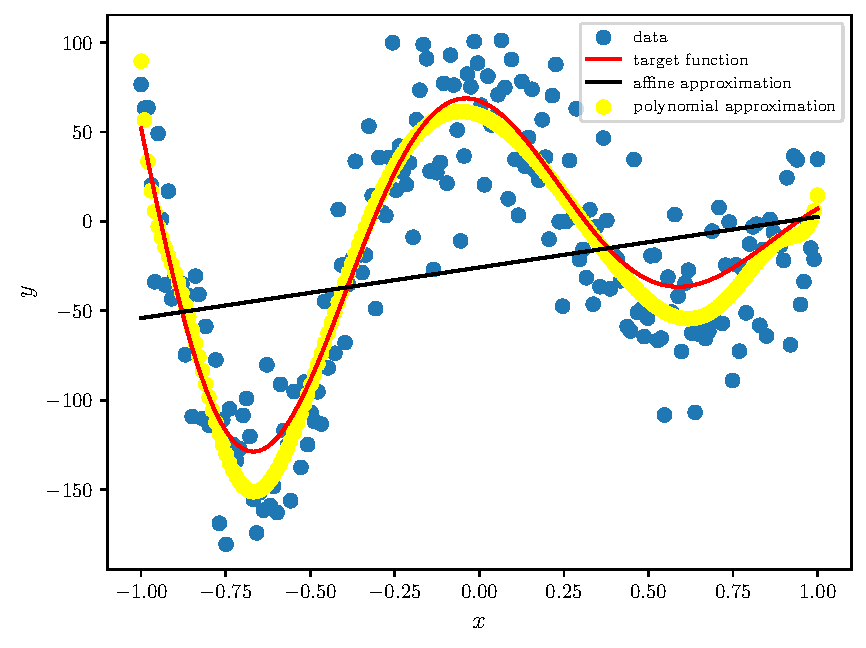
\includegraphics[width=0.8\textwidth]{Regression.pdf}
    \caption{A regression task; the goal is to fit noisy data (blue dots) assumed to be generated from a true function (solid red line). The data is fitted using an affine mapping (solid black line) and a polynomial mapping (solid yellow line).}
    \label{fig:regression}
\end{figure}   

\begin{boxedexample}[Classification] \complementary{\theexample}
    \label{ex:classification}
    We consider a classification problem of hand-written digits. The input to
    the problem is an $8 \times 8$ image of a hand-written digit, and the output
    should be the predicted value of the digit. Formally, we consider $x$ to be a
    random variable taking values in $[0, 16]^{8 \times 8} \subset
    \mathbf{N}^{8 \times 8}$, i.e., $x$ is a random variables in a matrix
    representation, where each matrix element takes an integer value between 0
    and 16. Here, the value of a certain matrix element represents its color,
    where 0 denotes black, and 16 denotes white. Let the target value $y$ be a
    random variable taking values in the discrete set $\{0,1,2,3,4,5,6,7,8,9\}$.
    To solve this supervised learning problem we consider as a hypothesis class
    the following multilayer perceptron:
    \begin{equation*}
        \mathfrak{H} = \bigl\{\text{softmax } w_2 \left(\sigma (w_1 \cdot x + b_1 ) \right) + b_2 ; w_1 \in \mathbb{R}^{\text{dh}, 8}, b_1 \in \mathbb{R}^{\text{dh}}, w_2 \in \mathbb{R}^{10, \text{dh}}, b_2 \in \mathbb{R}^{10}   \bigr\},
    \end{equation*}
    where dh is called the number of hidden units. In this class, the linear
    parameters are the weight matrices $w_1, w_2$ and the biases $b_1, b_2$.
    $\sigma$ is a nonlinear non-learnable function, often referred to by the \emph{activation function}. A common choice
    is the ReLU (Rectified Linear Unit) function
    \begin{equation*}
        \text{ReLU}(x) = \max(0, x)    
    \end{equation*}
 The softmax function (or layer) takes a set of real-valued input  and
 transforms it into a probability distribution over multiple classes. In our
 example we have ten classes and the softmax is given by
    \begin{equation*}
        \text{softmax}(z)_i = \frac{e^{z_i}}{\sum_{j=1}^{10} e^{z_j}}.
    \end{equation*}
    Therefore, the output of the hypothesis function is a probability distribution
    over the 10 classes. Concretly, the output is 10-dimensional, where each entry
    denotes the probability of the input image to represent a certain digit. 
    
    For facilitating the implementation we represent the target value as a one-hot
    vector. For example, given a target value 4, we represent it as the vector $y =
    (0,0,0,1,0,0,0,0,0,0)$. A suitable loss function for such problems is the
    categorical cross
    entropy
    function given by 
    \begin{equation*}
        l(h(x_i), y_i) = \sum_{c=0}^9 y_{i}^c \log(h(x_i)^c),
    \end{equation*}
    where $(x_i, y_i)$ is a specific training example. $y_{i}^c$ refers to the
    $c$-th entry of the one-hot vector representation of the target.

    Compute the training and test errors and study how they change when changing
    the number of hidden units or the number of layers.
\end{boxedexample}
  
\autoref{fig:regression} shows two hypotheses, one linear and one nonlinear, that we learned to fit the data in
\autoref{ex:regression}. The figure depicts an interesting phenomenon; a certain
hypothesis $h$ can fit the data too accurately; notice for example in
\autoref{fig:regression} that the polynomial-regression model fits badly local
minima of the target function. In these regions, it is optimized to fit the
noise. The outcome of such a result is that the polynomial-regression model will
fail to generalize well in these regions, i.e., it will have large error on
unseen data in these regions. This is called \emph{overfitting}.
On the other hand, the linear-regression model produces largely deviated results from
the data everywhere, and would, hence, also generalizes badly to unseen data.
This is called an \emph{underfitting} phenomenon. 

Think about the influence of the following factors on the underfitting and
overfitting:
\begin{itemize}
    \item Complexity of the model. For a polynomial-regression model this can be
    the degree of the polynomial. 
    \item Size of the dataset. For example, would adding more data decrease or
    increase underfitting?
\end{itemize}


\section{This Course}
In this section we introduce and motivate some questions that guide the
structure of this course.  
\subsection{Generalization Error and Minimization Principles}
In \autoref{ex:classification} and \autoref{ex:regression} we saw that a model
trained on a certain dataset $D_{\text{train}}$ is expected to generalize well on \emph{unseen}
data. This is a crucial difference from standard interpolation paradigms.
Formally, the training data is assumed to follow an unknown probability
distribution $P$, i.e., $D \sim P$. It is desirable that the learned model
not only performs well on $D$, but also on any other dataset $D_\text{test}$ that
also follows the distribution $P$. The problem is somehow ill-posed; \emph{how can one
fit a model to a training data $D$ and expect it to perform well on unseen data
$D_{\text{test}}$?}

One strategy to tackle this question is \emph{via} induction principle.
Formally, obtaining a hypothesis that minimizes the error over the whole
distribution, also known as the \emph{true risk}, is impossible. Instead, one
can do the next best thing. This is formally done by deriving an upper bound of
the true risk that includes, among other terms, the empirical risk, i.e., the
loss on the training data. Other terms include the so-called \emph{Rademacher
complexity}, a term which describes how complex the hypothesis class is. The
original task of minimizing the error over the whole probability distribution is
then replaced by the task of minimizing its upperbound. Such induction
strategies are called \emph{Empirical Risk Minimization Principles}. These
principles show that minimizing only the loss function of the training dataset
is not enough to obtain good generalization. One needs to regularize such loss
functions, i.e., to add some terms, whose minimization reduces the complexity of
the hypothesis class. This is directly linked to our previous discussion on
overfitting. 

The topic will be discussed in more detail in chapter 2.

\subsection{Hypothesis Classes and Approximation Capabilities}
In \autoref{ex:regression} and \autoref{ex:classification}, we have seen some
examples of hypothesis classes, such as the class of all affine mappings, the
class of polynomials up to a predefined degree, and the class of single-layer
neural networks. Another major hypothesis class is Kernel methods. Some
important questions here are as follows: given a certain learning problem, what
class do we use? Are we guaranteed to find an optimal solution in the chosen
class? Can we increase accuracy simply by increasing the complexity of our
class?

In chapter 3 we will study two important classes of models, neural networks
and kernel methods. We will survey some approximation properties of these classes and
perform error analysis for approximating important functions, such as continuous
functions, $L^p-$ functions and Sobolev functions. 

Moreover, we look with some detail at specific important application domains,
such as image recognition, and natural language processing.

\subsection{Curse of Dimensionality}
Assume that we want to optimize a potentially multi-variate unknown function $f:
\mathbb{R}^d \to \mathbb{R}$ using a dataset of
points sampled from it. Let $d=1$, i.e., assume for now that $f$ is uni-variate
and let our hypothesis class be a linear class. Let us denote by $T$ the
computational costs needed to achieve a certain accuracy $\epsilon$. It turns
out that $T$ grows exponentially with respect to $d$. In other words, the
computational costs required to achieve accuracy $\epsilon$ grow exponentially
with the dimension of the problem. This is known as the \emph{Curse of
Dimensionality} phenomenon.

Formally, when approximating an unknown function $f$ by a linear approximator
$\tilde{f}$, \emph{appriori} error estimates are often given by
\begin{equation*}
    \|f - \tilde{f}\| \leq c(d) \|f\|
\end{equation*}
where $\|.\|$ denotes some Sobolev norm of interest, and $c(d)$ is a constant that
scales exponentially with the dimension of the problem. See, for example, error
bounds for approximating Schwartz functions in the linear span of Hermite
functions~\cite{Lubich:QCMD}. 
\begin{boxedexample}[CoD:Fitting] \complementary{\theexample}
    \label{ex:CoD_fitting}
Consider fitting a dataset generated from the 1-dimensional target function
\begin{equation*}
    f(x) = \cos(2x) \exp(-x),
\end{equation*}
where you use the root-mean-squared error as a loss function and a
polynomial-regression model as a hypothesis class. What is the degree of the
polynomial necessary to achieve a training set error less than $10^{-5}$.
Similarly, study the same issue for fitting a dataset generated from the 2-dimensional target function
\begin{equation*}
    f(x,y) = \cos(2x y) \exp(-x).
\end{equation*}
\end{boxedexample}

In fact, this phenomenon is a major bottleneck for numerical methods to solve
differential equations, such as finite differences, finite volumes or spectral
methods. 
\begin{boxedexample}[CoD:Solving Schrödinger Equation] {\theexample}
    \label{ex:CoD_TISE}
Consider the following differential operator over $\mathbb{R}^d$
\begin{equation*}
    H = -\frac{1}{2} \bigl(\Delta + |x|^2 + \frac{1}{2} |x|^4 \bigr), 
\end{equation*}
where $\Delta$ denotes the Laplacian operator, and $|x| = \sqrt{\sum_{i=1}^d |x_i|^2}$. Its eigenvalue problem reads as follows: find all eigenpairs $(E_n, \psi_n)$
that satisfy
\begin{equation*}
    H \psi_n = E_n \psi_n. 
\end{equation*}
Assume we are interested only in the smallest eigenvalue $E_0$ and its
corresponding eigenfunction $\psi_0$. Consider approximating $\psi_0$
in the linear span of truncated Hermite functions $(\gamma_n)_{n=0}^\infty$,
i.e., 
\begin{align*}
    \psi_0 &\approx \tilde{\psi}_0 \\
    &= \sum_{n=0}^{N-1} c_n \gamma_n.
\end{align*}
Set $d=1$. How many Hermite functions $N$ are necessary to approximate $E_0$ to
a relative accuracy of $10^{-1}$? Repeat the same task for $d=2$ and 3. What do you
conclude? Answers are shown in \autoref{tab:ScaleDim}. For details on
calculations refer to~\cite{Saleh:thesis:2023}.
\end{boxedexample}
\begin{table}[t]
	\centering
	\caption[Size of basis to ensure convergence for an increasing problem dimensionality]{The size of a truncated Hermite basis $N$ that is required 
	to compute the smallest eigenvalue of the differential operator in
	\autoref{ex:CoD_TISE} in
	1,2 and 3 dimensions to a relative absolute error $< 10^{-1}$.}
	\begin{tabular}{lccccc}
		\hline\hline
		$d$ &1~&2~ &3		\\
		$N$   & 3 & 45 & 286  \\
		\hline\hline
	\end{tabular}
	\label{tab:ScaleDim}
\end{table}
There is evidence, however, that neural networks are less prone to the CoD
phenomenon. In other words, the computational scaling for using them to achieve
a certain accuracy on a given task do not scale dramatically with the dimension
of the problem. Characterizing such cases and providing rigorous understanding of
this is a crucial point in modern mathematical machine learning. We will touch
on this topic in chapter 4. Moreover, this topic will be of major
interest to us when considering physics-informed neural networks. 

\subsection{Approximating Highly-Oscillatory Functions}
The computational costs of approximation models, whether linear or nonlinear,
seem to increase exponentially with an increase in the oscillation of a target
function. This is a major bottleneck in some applications such as quantum
dynamics. An important example here is approximating solutions to
time-independent Schrödinger equations. Similar to \autoref{ex:CoD_TISE}, the
task here is to diagonalize a differential operator that describes a certain
quantum system. We look here at a specific example, where $H$ represents an
operator, that describes vibrational motions inside a molecule. Given a linear
numerical method to compute the eigenvalues, we look in \autoref{fig:osc} at the
relative accuracy of the
first 100 eigenvalues as a function of the truncation parameter $N$. It is clear
that larger eigenvalues are harder to approximate. Morever, increasing the
truncation parameter $N$ does a worse job for improving the accuracy of higher
eigenvalues than lower eigenvalues. This is partially because, larger
eigenvalues correspond to highly-oscillatory functions. For details on the
calculations see~\cite{Saleh:arXiv2308}.

\begin{figure}[htbp]
    \centering
    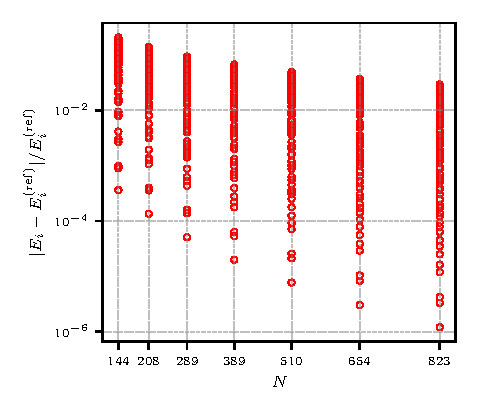
\includegraphics[width=0.8\textwidth]{H2S.pdf}
    \caption{The relative accuracy of the approximate first 100 eigenvalues of the vibrational Schrödinger equation for H$_2$S as a function of the truncation parameter $N$.}
    \label{fig:osc}
\end{figure}   
We will see in chapter 4 that neural-network approximation methods can
significantly improve approximation capabilities for highly-oscillatory functions.
\subsection{Validity of Occam's Razor and the Overparametrized Regime}
Theoretical and empirical results have demonstrated in the past 40 years that
Occam's Razor principle is valid when dealing with machine-learning problems:
\emph{Simple solutions are favored over unnecessarily complex ones.} Indeed,
one can see in, e.g., \autoref{ex:regression} that using a very high-order
polynomial can produce very good results on the training data, but fail badly to
produce sensible predictions on unseen data, resulting in an overfitting
phenomenon. However, new evidence implies that very complex neural networks seem
to generalize well on unseen data. In particular, many of the very successul
machine-learning models that we use in our everyday life are heavily
overparamterized, i.e., they have way more optimizable parameters than training
data. Neverthess they generalize well on unseen data. Understanding the
behavior of machine-learning models in this overparameterized regime is an
important research direction in modern machine learning.

\section*{What is not covered in this course}
The field of mathematical machine learning is huge and spans many standard
mathematical areas, ranging from (geometric) measure theory to statistical
learning theory, optimization theory and functional analysis. It is hence very
challenging to cover all topics in a master course. Here is a list of topics
that we do not cover in detail in this course and some references for
self-study. 

\begin{itemize}
    \item Optimizers and their convergence are largely ignored in this course.
    We use standard first order optimizers in all our numerical examples and do
    not comment on their convergence properties. 
    \item Bayesian learning models are largely marginalized.
    \item Unsupervised learning algorihtms such as clustering, and
    dimensionality reduction.
\end{itemize}

%----------------------------------------------------------------------------------------

\section*{Wait! What is what?}
Here is a list of questions that can help you check your understanding of key
concepts in this chapter.

\begin{enumerate}
    \item What are some examples of hypothesis classes? Which of them are
    linear or nonlinear approximation methods?
    \item What loss functions do you know for regression and classification
    tasks? Can you think of other examples than the ones mentioned in this
    chapter?
    \item For a fitting problem, can we get more accurate results by increasing
    the complexity of the hypothesis class?
    \item How are the computational costs related to the dimension of the
    problem? 
\end{enumerate}


% Chapter 1
% !TeX spellcheck = en_US 
\chapter{Statistical Learning Theory} % Main chapter title

\label{Chapter2} % For referencing the chapter elsewhere, use \ref{Chapter1} 
\setcounter{chapter}{2}
%----------------------------------------------------------------------------------------
In the previous chapter we have observed the phenomenon of overfitting; a model
trained to minimize the empirical risk on a training dataset can still fail to generalize
well over unseen dataset. A fundamental question in statistical learning theory is how to design
hypothesis classes that do not overfit.  

We will see in this chapter that restricting the complexity of the hypothesis classes can help
reduce the overfitting. First, we start by looking at finite hypothesis classes
and show that they do not overfit. This result will also motivate a notion of statistical learning, that of \emph{probably approximately correct
(PAC)} learning. However, finiteness of the hypothesis class is, indeed, a very
restricting condition. We will discuss other measures of the complexity of a
hypothesis class, such as the \emph{Vapnik-Chervonenkis (VC) dimension} and the
\emph{Rademacher complexity}. At the end of this chapter, we will discuss what
these theoretical results imply for the design of machine learning algorithms and
link to the concept of \emph{overparameterization}, which is a hot topic in the field of deep learning.

The reader is referred to~\cite{Shalev:ML:2014} and~\cite{Shapire:ThML2019} for more details. 

We start this section by recalling some basic definitions of probability
measure theory.
\section{Probability Measure Theory}
As we have seen in \nameref{Chapter1}, training datasets are treated as random
variables. This makes the following tools from probability theory essential. 

Let $(\Omega,\mathcal{A}, \mathbb{P})$ be a probability measure space, where $\Omega \subseteq \mathbb{R}$. 
It is common to refer to any $A \in \mathcal{A}$ by an \emph{event}. An event
$A$ s.t. $\mathbb{P}(A)=1$ is said to happen \emph{almost surley.}

Important probability measures are those induced by measurable transformations in the following way. 
\begin{definition}[Push-forward Measure]
	Given two measurable spaces $(\Omega_1, \mathcal{A}_1)$, $(\Omega_2, \mathcal{A}_2)$ and a measurable mapping $h:\Omega_1 \to \Omega_2$ 
	the \emph{push-forward measure} of a measure $\mathbb{P}$ on $(\Omega_2, \mathcal{A}_2)$ is 
	$$
	h_\#\mathbb{P} (A) := \mathbb{P} (h^{-1}(A)) \quad  \forall A \in \mathcal{A}_2.
	$$
	The push-forward measure is sometimes denoted by $\mathbb{P} h^{-1}$.
\end{definition}

We look now at a special kind of measurable mappings and the measures they induce.
\begin{definition}[Real Random Variables and Distributions]
	\label{def:RV}
	\begin{enumerate}[(i)] Let $(\Omega,\mathcal{A}, \mathbb{P})$ be a probability measure space.
		\item A measurable mapping $V: \Omega \to \mathbb{R}$ is called a \emph{real random variable}.
		\item The push-forward measure $\mathcal{P}_V := V_\# \mathbb{P}$ induced by a real random variable $V$ 
		is called the \emph{(probability) distribution of $V$}.		
	\end{enumerate}
\end{definition}
A mapping $V: \Omega \to \mathbb{R}^n$ for $n>1$ is usually referred to as a
\emph{random vector}. In our treatment we will refer to $V$ by a random variable
for any $n\geq 1$. 
\begin{definition}[Expected Value]
	\begin{itemize}
		\item The expected value of a random variable $X: \Omega \to
		\mathbb{R}$, denoted by $\mathbb{E}[X]$
		is defined as:
		\begin{align*}
			\mathbb{E}[X] &:= \int_\Omega X(\omega) \ d\mathbb{P}(\omega) \\
			& = \int_\mathbb{R} x \ d\mathcal{P}_X(x),
		\end{align*}
		where $\mathcal{P}_X$ is the pushforward-measure of $X$.
		\item Similarly, the expected value of a measurable mapping $g:
		\mathbb{R}\to \mathbb{R}$ as a function of the random variable $X$ is given by 
		\begin{align*}
			\mathbb{E}[g(X)] &:= \int_\Omega g(X)(\omega) \ d\mathbb{P}(\omega) \\
			& = \int_\mathbb{R} g(x) \ d\mathcal{P}_X(x).
		\end{align*}
		Sometimes, one writes $\mathbb{E}[g] = \mathbb{E}_{x \sim \mathcal{P}_x}[g]$
		to highlight the measure on $\mathbb{R}$ against which one integrates.
	\end{itemize}
\end{definition}


\begin{definition}[Independent Events]
Two events $A,B$ are said to be \emph{independent} if $$\mathbb{P}(A \cap B) = \mathbb{P}(A)\mathbb{P}(B).$$ Given 
an index set $I$, consider the family $A_i \in \mathcal{A}$ for $i \in I$. The
family $(A_i)_{i\in I}$ of events is said to be \emph{independent}
if $$\mathbb{P}(\cap_{j \in J} A_j) = \prod_{j \in J} \mathbb{P}(A_j) \quad \forall J \subset I.$$	
\end{definition}

The independence of events (i.e., sets) can be generalized to independence of
families of sets. 
\begin{definition}[Independence of Families of Sets]
        Let $I$ be an index set and consider $\mathcal{E}_i \subseteq \mathcal{A}$ for all $i \in I$.
        The family $(\mathcal{E}_i)_{i \in I}$ is called \emph{independent} if, for any finite subset 
        $J \in I$ and any choice of $E_j \in \mathcal{E}_j, j \in J$, one has 
        $$
        \mathbb{P}(\cap_{j \in J} E_j) = \prod_{j \in J} \mathbb{P}(E_j).
        $$
\end{definition}
The following is an important family of random variables that one often encounters 
in machine learning and statistics. 
\begin{definition}[Independent and Identically Distributed Random Variables]
	\label{def:iid}
	Let $I$ be an index set and $(V_i)_{i \in I}$ be a family of real random 
	variables. Endow $\mathbb{R}$ with the Borel $\sigma$-algebra $\mathcal{B}$.
	\begin{enumerate}[(i)]
		\item The family $(V_i)_{i \in I}$ is said to be \emph{identically distributed} if 
		$$\mathcal{P}_{V_i} = \mathcal{P}_{V_j} \quad \text{ for all } i, j \in I.$$
		\item The family $(V_i)_{i \in I}$ is said to be \emph{independent} if the 
		family of generated $\sigma$-algebras $\bigl(\sigma(V_i) \bigr)_{i\in I}$, where 
		$\sigma(V_i) = V_i^{-1}(\mathcal{B})$ is independent.
	\end{enumerate}
A family of real random variables satisfying both conditions is said to be
\emph{independent and identically distributed (i.i.d.)}.
In such a case set $\mathcal{P} = \mathcal{P}_{V_i}$. \end{definition}

\section{A Formal Setting of Learning}
\label{sec:formal_learning}
We start by defining the standard setting of supervised learning. In our
treatment, we will not use this very general setting. We will be imposing restrictions, for
example, by considering only binary classification problems, or by using special
loss functions. Nevertheless, it is useful to see the general setting first.

Let $z = (x, y)$ be a random variable where $x: \Omega \to \mathbb{X} \subseteq
\mathbb{R}^n$ and $y: \Omega \to \mathbb{Y} \subset \mathbb{R}$. Denote by
$\mathcal{P}$ the probability distribution of $z$ and by $\mathcal{P}_x$ the
marginal probability distribution corresponding to the random variable $x$.
Further, we set $\mathbb{Z} := \mathbb{X} \times \mathbb{Y}$ \footnote{Do not
confuse the notation with the set of integers.}. We denote by $p(z)$ and $p(x)$
the probability density functions of $z$ and $x$, respectively. These two
densities are related by the formula $p(z) = p(x)p(y|x)$.

Given a hypothesis class $\mathfrak{H}$ of functions $h: \mathbb{X} \to \mathbb{Y}$ and a loss function $l:\mathbb{Y}^2 \to \mathbb{R}_{>0}$, the goal of a supervised-learning
algorithm is to solve 
\begin{equation*}
    \underbrace{R_{\mathcal{P}}(h) := \int_{\mathbb{Z}} l(y, h(x)) \ d \mathcal{P}}_{\text{True risk}} \longrightarrow \min_{h \in \mathfrak{H}} \implies h^\star, 
\end{equation*}
that is, to minimize the \emph{true risk}. Note that the true risk is also called the
\emph{generalization error}. However, one only has access to a finite
realiazation of the random variable $z$, i.e., to a training set $D=\{(x_i,
y_i)_{i=1}^m\}$. A reasonable thing to do is, hence, to minimize a
finite/empirical representation of the true risk, i.e., to solve
\begin{equation*}
    \underbrace{\hat{R}_{\mathcal{P}} (h) := \sum_{(x,y) \in D} \frac{1}{|D|}l(y, h(x)) }_{\text{Empirical risk}} \longrightarrow \min_{h \in \mathfrak{H}} \implies \hat{h}^\star.
\end{equation*}

A learning algorithm that replaces the original task of minimizing the true risk
by the task of minimizing the empirical risk is called an \emph{empirical risk
minimization (ERM) learner} or
is said to be using the \emph{ERM learning rule}. To highlight the dependence of
the empirical risk on the training data, we sometimes write $\hat{R}_{\mathcal{P}}(h;D)$.

One of the main problems of statistical learning theories is to study the
validity of approximating $h^*$ by $\hat{h}^*$. In particular, under what
conditions on the hypothesis class does $\hat{h}^*$ have a small generalization error?
In the next section, we will see that the finiteness of the hypothesis class is
a sufficient condition to this end. Is it necessary though?

\section{Probably Approximately Correct Learning}

We start this section by looking closely at the problem of overfitting and show that
finite classes do not overfit. Our results to this end motivate a notion of
statistical learning that we discuss.

For this section, we will adopt the setting defined in
\autoref{sec:formal_learning} and further assume that $\mathbb{Y} = \{0,1\}$,
i.e., we restrict ourselves to the binary classification case. Moreover, we
assume that $y$
is generated from $x$ by the deterministic functional relation $y=f(x)$, where $f: \mathbb{X}
\to \{0,1\}$. Unless otherwise stated, we will set the loss function to be the 0-1 loss
which
we define as follows.
\begin{equation*}
    l(y, h(x)) :=
    \begin{cases}
         & 1: \ h(x) \neq y \\
        & 0: \ \text{otherwise}.
    \end{cases}	
\end{equation*}
Note that in this case, the true and empirical risks simplify to
$$
R_{\mathcal{P}}(h) = \mathcal{P}_x \bigl(\{x: h(x) \neq y\} \bigr)
$$
$$
\hat{R}_{\mathcal{P}}(h) = \frac{1}{m} | \{x: h(x) \neq y\} |
$$

Moreover, we restrict ourselves to working under the  
 \emph{realizability assumption}, i.e., that
there exists $h^* \in \mathfrak{H}$ s.t. $R_{\mathcal{P}}(h^*) = 0$. Note that
this assumption implies that the empirical risk of the hypothesis obtained by
the ERM rule is zero, i.e., $\hat{R}(\hat{h}^*) = 0$ with probability 1 over the
choice of the training data. In other words, the realizability assumption
implies that the ERM rule provides a hypothesis that is \emph{consistent} on the
training data. To see this, note that $R_\mathcal{P}(h^*)=0$ implies
that $\hat{R}_\mathcal{P}(h^*;D)=0$ with probability 1 over the choice of a
dataset $D$ that is i.i.d. generated by $\mathcal{P}$. In turn, this implies
that $\hat{R}_\mathcal{P}(\hat{h}^*;D)=0$ with probability 1 over the choice of
$D$ since $\hat{R}_\mathcal{P}(\hat{h}^*;D) \leq \hat{R}_\mathcal{P}(h^*;D)$ by
the definition of the ERM rule.

\subsection{Finite Hypothesis Classes do not Overfit}
The goal in this section is to show that we won't encounter an overfitting
problem if the hypothesis class has finitely many elements. We will deal with
the overfitting problem in an approximate manner, i.e., we will say that a
hypothesis $h$ does not overfit if $R_\mathcal{P}(h)\leq \epsilon$ for some
small $\epsilon>0$.

In what follows, given a dataset $D$, we denote by $D|_x$ the input of the
dataset, i.e., $D|_x=\{x_i: i=1,\dots,m\}$. Note that since each $x\in D|_x$ is a
random variable with a distribution $\mathcal{P}_x$, the dataset $D|_x$ has distribution $\mathcal{P}^m_x$ over $\mathbb{X}^m$.

\begin{lemma}
	\label{lem:PAC_fh}
		Under the realizability assumption and
		for accuracy $\epsilon >0$ it holds that 
		$$
		\mathcal{P}^m_x\bigl(\{D|_x: R_\mathcal{P}(\hat{h}^*) > \epsilon\} \bigr) \leq |\mathfrak{H}| e ^{-\epsilon m}.
		$$
	\end{lemma}
	In words; the probability of sampling $m$ training data points and
	obtaining a learner $\hat{h}^*$ by the ERM rule that does not generalize well is
	upperbounded. Note that this upperbound is finite if the cardinality of
	$\frak{H}$ is finite. Also note that 
	$$
	\mathcal{P}^m_x\bigl(\{D|_x: R_\mathcal{P}(\hat{h}^*) > \epsilon\} = \mathbb{P}_{D|_x \sim \mathcal{P}^m_x} \bigl( \{ R_\mathcal{P}(\hat{h}^*) > \epsilon \}\bigr). 
	$$
\begin{proof}
    We start by defining the set $\mathfrak{H}_b$ of bad hypotheses, i.e., the
    set of all hypotheses that lead to a generalization error $> \epsilon$,
    $$
    \mathfrak{H}_b := \{h \in \mathfrak{H} \text{ s.t. } \mathbb{R}_\mathcal{P} (h) > \epsilon\}.
    $$
    Next, we define the set of misleading training data, i.e., the set of all
    training datasets of cardinality $m$, on which there is at least one
    hypothesis that produces zero training error and a generalization error $>
    \epsilon$,
    $$
    M:= \{D|_x: \ |D|_x|=m, \text{ and s.t. there exists }h  \in \mathfrak{H}_b : \ \hat{R}_\mathcal{P}(h;D)=0 \}.
    $$
    Note that the realizability assumption implies that
    $\hat{R}_\mathcal{P}(\hat{h}^*)=0$ as discussed before. This in turn implies
    that $\{D|_x: R_\mathcal{P}(\hat{h}^*) > \epsilon\} \subseteq M$. It thus
    follows that 
	\begin{align*}
		\mathcal{P}^m_x\bigl(\{D|_x: R_\mathcal{P}(\hat{h}^*) > \epsilon\}\bigr) &\leq \mathcal{P}^m_x(M)\\
		&\leq \sum_{h \in \mathfrak{H}_b} \mathcal{P}^m_x\bigl(\{D|_x: \hat{R}_\mathcal{P}(h;D)=0\}\bigr)\\
		&= \sum_{h \in \mathfrak{H}_b} \prod_{i=1}^m \mathcal{P}_x\bigl(\{x: h(x) = y\}\bigr)\\
		&= \sum_{h \in \mathfrak{H}_b} \prod_{i=1}^m (1-R_\mathcal{P}(h)) \quad {\color{mildred} \text{(definition of true risk)}}\\
		&\leq \sum_{h \in \mathfrak{H}_b} (1-\epsilon)^m \quad {\color{mildred} \text{(since } h \in \mathfrak{H}_b)}\\
		&\leq |\mathfrak{H}_b| (1-\epsilon)^m \\
		&\leq |\mathfrak{H}| (1-\epsilon)^m \\
		&\leq |\mathfrak{H}| e^{-\epsilon m}.
	\end{align*}	
\end{proof}
The above lemma shows that the probability of overfitting is exponentially small
with the size of the training data. It also provides us with a way to find the
minimal amount of training data that guarantees a small generalization error.
    \begin{coro}
		\label{Coro:finite_hypo}
		Let $\mathfrak{H}$ be a finite hypothesis class. Let $\delta \in (0,1)$ be a confidence parameter and $\epsilon \in
		(0,1)$ be an accuracy parameter. Let $m$ be an integer that satisfies
		$$
		m \geq \frac{1}{\epsilon} \log(|\mathfrak{H}|/\delta).
		$$ 	
		Under the realizability assumption it holds that 
		$$
		\mathbb{P}_{D|_x \sim \mathcal{P}^m_x} \bigl( \{ R_\mathcal{P}(\hat{h}^*) > \epsilon \}\bigr) \leq \delta.
		$$
		In other words, 
		$$
		R_\mathcal{P}(\hat{h}^*) \leq \epsilon
		$$
		holds with probability of at least $1-\delta$ over the choice of the
		training data $D$.
	\end{coro}
	Note that this result holds for any labeling function $f$ and any
	distribution $\mathcal{P}_x$. 
    \begin{proof}
        Follows straight-forwardly from the previous lemma.
    \end{proof}
The results we proved so far show that finite hypothesis classes do not overfit.
Here, overfitting is defined in an \emph{approximate sense} controlled by parameter
$\epsilon$. The results guarantee that the ERM rule provides a hypothesis
that generalizes well in a \emph{probabilistic sense}. The probability here is
controlled by a parameter $\delta$. This motivates the following definition.

    \begin{definition}
		A hypothesis class $\mathfrak{H}$ is PAC learnable if there exist a
		function $m_\mathfrak{H}: (0,1)^2 \to \mathbb{N}$ and a learning
		algorithm with the following properties
		\begin{itemize}
			\item for every $(\epsilon, \delta) \in (0,1)^2$
			\item for every distribution $\mathcal{P}_x$ over $\mathbb{X}$
			\item for every labeling function $f: \mathbb{X} \to \{0,1\}$
		\end{itemize}
		s.t. if the realizability assumption holds, when running the learning
		algorithm on $m \geq m_\mathfrak{H}(\delta, \epsilon)$ i.i.d. samples
		generated by $\mathcal{P}_x$ and labeled by $f$, the algorithm returns a
		hypothesis $h$ such that 
		$$
		R_\mathcal{P}(h) \leq \epsilon
		$$ 
		with probability of at least $1-\delta$ over the choice of the samples.
	\end{definition}

    \begin{definition}[samples complexity]
		The sample complexity of leaning a hypothesis class $\mathfrak{H}$ is
		the minimal integer that satisfies the requirement of PAC learnability
		with accuracy $\epsilon$ and confidence $\delta$.
	\end{definition}
	With these definitions we can restate our corollary in the following manner.
	\begin{coro}
		Every finite hypothesis calss is PAC learnable with sample complexity 
		$$
		m \leq \lceil \frac{1}{\epsilon} \log(|\mathfrak{H}|/\delta) \rceil
		$$
	\end{coro}
One may wonder whether the finiteness of the hypothesis class is a necessary
condition for PAC learnability. We will see now that this is indeed not the
case. For example, we consider here the class of threshold functions. 
\begin{definition}[Class of Threshold Functions]
	$\mathfrak{H} := \{h_a:\mathbb{R}\to \{0,1\}, h_a(x)= \mathbf{1}_{x <a} ,\  a\in \mathbb{R}\}$
\end{definition}	
In words, this class consists of all functions that assign 1 to all inputs that
are smaller than a threshold $a$ and 0 otherwise. The class of threshold
functions has infinite cardinality. However, we will see that this class is PAC learnable.
\begin{lemma}
The class of threshold functions	$\mathfrak{H}$ is PAC-learnable using the ERM rule with sample complexity of
	$m_\frak{H} \leq \lceil \frac{1}{\epsilon}\log (2/\delta)\rceil$.
\end{lemma}
\begin{proof}
	It suffices to show that 
	$$
	\mathbb{P}_{D|_x \sim \mathcal{P}^m_x} \bigl( \{ R_\mathcal{P}(\hat{h}^*) > \epsilon \}\bigr) \leq 2 \exp(-\epsilon m).
	$$
	To prove this note that we work under the realizability assumption. Hence,
	it is possible to find a hypothesis $\hat{h}^* = h_{\hat{a}^*}$ that is
	consistent with the training data. 
	
	Let $a^*$ be the threshold of the labeling function $f$. Let $a^* _r >a^*$ be such that $\mathbb{P}_{x \sim \mathcal{P}_x}\bigl(x \in (a^*,
	\hat{a}^*_r)\bigr)= \epsilon$. Similarly, let $a^*_l <a^*$ be such
	that $\mathbb{P}_{x \sim \mathcal{P}_x}\bigl(x \in (\hat{a}^*_l, a^*)\bigr)=
	\epsilon$. Notice that picking datapoints that are outside the interval
	$(a^*_l, a^*)$ or outside $(a^*, a^*_r)$ is a sufficient condition for picking training datasets that lead to a bad
	hypothesis. Formally
	\begin{align*} 
	\mathbb{P}_{D|_x \sim \mathcal{P}^m_x} \bigl( \{ R_\mathcal{P}(\hat{h}^*) > \epsilon \}\bigr) &\leq \mathbb{P}_{D|_x \sim \mathcal{P}^m_x} \bigl(\{\forall x \in D|_x,  x \notin (a^*_l, a^*) \vee x \notin (a^*, a^*_r)\}\bigr) \\
	&\leq \underbrace{\mathbb{P}_{D|_x \sim \mathcal{P}^m_x} \bigl(\{\forall x \in D|_x,  x \notin (a^*_l, a^*) \}\bigr)}_{\text{term} 1} + \mathbb{P}_{D|_x \sim \mathcal{P}^m_x} \bigl(\{\forall x \in D|_x,  x \notin (a^*, a^*_r)\}\bigr). 
	\end{align*}
	Note that 
	\begin{align*}
		\text{term }1 &\leq \mathbb{P}_{D|_x \sim \mathcal{P}^m_x} \bigl(\{x_1 \notin (a^*_l, a^*) \wedge x_2 \notin (a^*_l, a^*) \wedge \dots \wedge x_m \notin (a^*_l, a^*) \}\bigr)\\
		&= \prod_{i=1}^m \mathbb{P}_{x \sim \mathcal{P}_x} \bigl(x \notin (a^*_l, a^*)\bigr)\\
		&= (1-\epsilon)^m.
	\end{align*}
	The claim follows by doing the same inequality for the second term and using $(1-\epsilon)^m \leq \exp(-\epsilon m)$.
\end{proof}
In summary, our results show that finiteness of the hypothesis class is not a
good condition for characterizing PAC learnability, since infinite classes can
be PAC learnable. We thus move in the next section to introduce a better measure
of the complexity of a hypothesis class.

\subsection{Vapnik-Chervonenkis Dimension}
The Vapnik-Chervonenkis (VC) dimension is a measure of the complexity of a
hypothesis class. The intuition behind this measure is to define the richness of
a class with respect to a given dataset. For example, a class of threshold
functions is infinite dimensional. However, given a dataset $D$ of only one
point $x \in \mathbb{R}$, the whole class of threshold functions can give this
datapoint only two
different values, either 0 if the hypothesis has a threshold lying to the
left of the datapoint, or 1 otherwise. Now consider a dataset
of two points. The class of threshold functions can label these two points in three
different ways, (0,0), (1,0) or (1,1). However, the hypothesis class of threshold
functions cannot represent the labeling (0,1). Hence, the class of threshold
functions cannot exhaust all the possible labeling of a dataset of two
points. This is indeed the motivation behind the following definitions.

\begin{definition}[Restriction of $\mathfrak{H}$ to $C$]
	Let $\frak{H}$ be a class of functions from $\mathbb{X}$ to $\{0,1\}$
	and let $C = \{x_1, \dots, x_m\} \subset \mathbb{X}$. The restriction of
	$\mathfrak{H}$
	to $C$ is the set of functions from $C$ to $\{0,1\}$ that can be derived from
	$\mathfrak{H}$. That is, 
	$$
	\mathfrak{H}_C := \{(h(x_1), \dots, h(x_m)): h \in \mathfrak{H}\}.
	$$	
	 \end{definition}
	 If $\mathfrak{H}_C$ is the set of all functions from $C$ to $\{0,1\}$
	 we say that $\mathfrak{H}$ shatters $C$. Formally we write as follows.
	 \begin{definition}[Shattering]
		A hypothesis class $\mathfrak{H}$ shatters a finite set $C \subset
		\mathbb{X}$
		if $|\mathfrak{H}_C|= 2^{|C|}$.
	 \end{definition}
	 According to this definition we observe that the class of threshold
	 functions shatters a set of one point but does not shatter a set of two
	 points, because it does not exhaust all of its possible labelings.

	 The following definition quantifies the number of different labelings that a
	 hypothesis class can provide for a dataset of fixed size.
	 \begin{definition}[Growth Function]
		Let $\mathfrak{H}$ be a hypothesis class. The growth function of
		$\mathfrak{H}$, denoted by $\tau_\mathfrak{H} :\mathbb{N} \to \mathbb{N}$ is defined as 
		$$
		\tau_\mathfrak{H}(m) := \max_{C \subset \mathbb{X}: |C|=m}|\mathfrak{H}_c|
		$$
	\end{definition} 
	In words; $\tau_\mathfrak{H}(m)$ is the maximum number of different functions
	from a set $C$ of size $m$ to $\{0,1\}$ that can be obtained
	by restricting $\mathfrak{H}$ to $C$.

	It turns out that the growth function is a good quantity to measure the
	complexity of a hypothesis class, since a bounded growth function implies
	PAC learnability.
	\begin{thm}
		\label{thm:PAC_gf}
		Let $\delta \in (0,1)$ be a confidence parameter and $\epsilon \in
		(0,1)$ be an accuracy parameter. Let $m$ be an integer that satisfies
		$$
		\epsilon \geq  \frac{1}{m}\log(|\tau_\mathfrak{H}(2m)|/\delta).
		$$ 	
		Under the realizability assumption it holds that 
		$$
		\mathbb{P}_{D|_x \sim \mathcal{P}^m_x} \bigl( \{ R_\mathcal{P}(\hat{h}^*) > \epsilon \}\bigr) \leq \delta.
		$$
	\end{thm}	 
	Note that this result is very similar to \autoref{lem:PAC_fh}. The main difference is that the growth function is used instead of the cardinality of the hypothesis class.
	\begin{proof}
		To prove the result it suffices to show that 
		$$
		\mathcal{P}^m_x\bigl(\{D|_x: R_\mathcal{P}(\hat{h}^*) > \epsilon\} \bigr) \leq 2 \tau_\mathfrak{H}(2m) 2^{-\epsilon m/2}.
		$$
		Given a hypothesis function $h$ we define the quantity $M(h;D)$ as the
		number of errors that $h$ makes on the dataset $D$. Since we are using
		the 0-1 loss we note that $\hat{R}_\mathcal{P}(h;D) = M(h;D)/m$. 
	We define the event $B$ as the event that a hypothesis
	 is consistent with the training data but does not generalize well, i.e., 
$$
B : \exists h \in \mathfrak{H}: M(h;D) = 0 \wedge R_\mathcal{P}(h) > \epsilon.
$$
To have an empirical estimate of the true risk we assume that we have access to
a test set $D'$ of size $m$ that is i.i.d. generated by $\mathcal{P}_x$. We now
define the event $B'$
$$ 
B' : \exists h \in \mathfrak{H}: M(h;D) = 0 \wedge M(h;D') > \epsilon m/2.
$$
Now consider the following experiment. For each element $x \in D|_x$ and $x' \in
D'|_x$ we flip a fair coin. If the coin lands heads we swap $x$ with $x'$.
Otherwise we do not swap. We denote the resulting datasets by $T$ and $T'$. We
now define the event $B''$ as follows
$$ 
B'' : \exists h \in \mathfrak{H}: M(h;T) = 0 \wedge M(h;T') > \epsilon m/2.
$$
We now claim that
$$
\mathbb{P}(B) \underbrace{\leq}_{*_1} 2 \mathbb{P}(B') \underbrace{=}_{*_2} 2 \mathbb{P}(B'') \underbrace{\leq}_{*_3} 2 \ \tau_\mathfrak{H}(2m) 2^{-\epsilon m/2}.
$$
Proving this claim would complete the proof. We now prove the inequality1
$*_1$,

Note that 
\begin{align*}
	\mathbb{P}(B') &\geq \mathbb{P}(B' \wedge B) \\
	&= \mathbb{P}(B'|B) \mathbb{P}(B)	
\end{align*}
The claim now follows from the fact that $\mathbb{P}(B'|B) \geq 1/2$ if $m \geq 8/\epsilon$. While we
will not formally prove this result, here is the intuition behind it. Assume
that the event $B$ has occurred. This means that there is a hypothesis $h$ that
is consistent with the training data but does not generalize well. Now consider
$M(h;D')$ as a random variable and note that $\mathbb{E}_{D'|_x \sim
\mathcal{P}^m_x} M(h;D') = R_\mathcal{P}(h) m$. Since $R_\mathcal{P}(h) >
\epsilon$ we have that $\mathbb{E}_{D'|_x \sim \mathcal{P}^m_x} M(h;D') >
\epsilon m/2$. Hence, the probability of $B'$ is equivalent to the probability of
the random variable $M(h;D')$ being larger than a lower bound to its expected
value. The desired result is based on the use of a measure-concentration
inequality, i.e., an inequality that study the convergence of an
empirical
average of a random variable to its true expected value.

To see the inequality $*_2$ note that the samples $D, D'$ are i.i.d. generated
by $\mathcal{P}_x$. Since $T,T'$ were generated by equally likely permutations,
we have that $T,T'$ are also i.i.d. generated by $\mathcal{P}_x$. Hence, the
probability of $B''$ is the same as the probability of $B'$.

The inequality $*_3$ follows from the application of the law of total
expectation which states that for two random variables $X,Y$ it holds that
$\mathbb{E}(X) = \mathbb{E}(\mathbb{E}(X|Y))$. Note that the probability of some
event $A$ can be written as the expected value of the indicator function of $A$.
It hence follows that 
$$
\mathbb{P}_{D, D' \sim \mathcal{P}_x^{2m}}(B'') = \mathbb{E}_{D, D' \sim \mathcal{P}_x^{2m}} \mathbb{P}(B''|D,D').
$$ 

Now let $\mathfrak{H}'$ be a hypothesis class containing one representative for
each different labeling of $\mathfrak{H}$ of $D, D'$. 
We have that 

\begin{align*}
\mathbb{P}(B''|D, D') & = \mathbb{P}(\exists h \in \mathfrak{H}: \underbrace{M(h;T) = 0 \wedge M(h;T') > \epsilon m/2}_{:=b(h)}|D, D')\\ 
&= \mathbb{P}(\exists h \in \mathfrak{H}': b(h)|D, D')\\
&\leq \sum_{h \in \mathfrak{H}'} \mathbb{P}(b(h)|D, D')\\
&\leq |\mathfrak{H}'| 2^{-\epsilon m/2}\quad \text{\color{mildred} assume }{\color{mildred} \mathbb{P}(b(h)|D, D') \leq 2^{-\epsilon m/2}}\\
&\leq \tau_\mathfrak{H}(2m) 2^{-\epsilon m/2}.
\end{align*}
We prove the assumption $\mathbb{P}_{D, D' \sim \mathcal{P}_x^{2m}}(b(h)|D, D') \leq 2^{-\epsilon m/2}$ by
considering three different cases. For a fixed $h$, we note that $D, D'$ already
occurred. Hence, the only randomness is coming from the random permutation
process to construct $T, T'$.

Assume for the first case that there exists an index $i$ s.t. $h$ makes a mistake
on both $x_i \in D|_x$ and $x'_i \in D'|_x$. In this case, it is not possible to have $M(h;T)=0$.
Hence, the event $b(h)$ occurs with probability 0.

For the next two cases define $r$ to be the number of pairs $(x_i, x'_i), x_i
\in D|_x, x_i' \in D'|_x$ where $h$ is wrong on exactly one between the two,
i.e., either on $x_i$, or on $x'_i$.

Consider for the second case $r < m \epsilon/2$. Even if we get lucky enough and
all elements on which $h$ is correct end up in $T$, we will not have enough
datapoints to satisfy the condition $M(h;T') > \epsilon m/2$. Hence, the event $b(h)$ occurs with probability 0.

For the third case consider $r \geq m \epsilon/2$. In this case, we need that
all the coin flips end up in the correct way to have zero mistakes in $T$ and
all mistakes in $T'$. Since the coin flips are independent and fair, we have
that
$$
\mathbb{P}(b(h)|D, D') = 2^{-r} \leq 2^{-m \epsilon/2}.
$$

\end{proof}
	Due to the combinatorial nature of the growth function, its asymptotic
behavior is not obvious. Getting hold of it would provide a better bound in
\autoref{thm:PAC_gf}. We will now introduce the more intuitive quantity of the
VC-dimension, which will enable us to calculate how many datapoints we need to get
PAC learnability with a hypothesis class of infinite cardinality.	
	\begin{definition}[VC (Vapnik-Chervonenkis) dimension]
		The VC dimension of a hypothesis class $\mathfrak{H}$, denoted
		$\text{VC-dim}(\mathfrak{H})$ is the cardinality of the largest set $C$ that
		can be shattered by $\mathfrak{H}$.  
	\end{definition}
	\begin{example}
		To show that a finite hypothesis class has a VC-dimension d, it suffices to show that there exists a set of size $d$ that can be shattered by the hypothesis class and that there exists no set of size $d+1$ that can be shattered by the hypothesis class.
		\begin{itemize}
			\item The VC dimension of threshold functions is 1.
			\item Consider the following hypothesis class
			$$
			\mathfrak{H} = \{h: h(x) = \mathbf{1}_{x \in (a,b)}, a<b, a,b\in \mathbb{R}\}.
			$$ 
			The VC dimension of this class is 2.
		\end{itemize}
	\end{example}
	The previous examples may convey the idea that the VC dimension of a certain
	class equals the number of free parameters that the class has. This is not
	always the case. For example, the VC dimension of the class 
	$$
	\mathfrak{H} = \{h(x) = \sin(\theta x): \theta \in \mathbb{R}\}
	$$
	is infinite.

	The following lemma allows us to replace the growth function by the VC-dimension in \autoref{thm:PAC_gf}.
	\begin{lemma}[Sauer's lemma]
		Let $\mathfrak{H}$ be a hypothesis class. If 
		\begin{itemize}
			\item $VC-dim(\mathfrak{H})< \infty$ then $\tau_\mathfrak{H}=O(m^d)$
			for all $m\in \mathbb{N}$.
			\item $VC-dim(\mathfrak{H})=\infty$ then $\tau_\mathfrak{H}=2^m$
			for all $m\in \mathbb{N}$.
		\end{itemize}
	\end{lemma}
		\begin{coro}
			Let $\delta \in (0,1)$ be a confidence parameter and $\epsilon \in
			(0,1)$ be an accuracy parameter. Assume
			$\text{VC-dim}(\mathfrak{H})=d<\infty$. Let $m$ be an integer that
			satisfies
			$$
			\epsilon \geq  C \frac{d \log m + \log(1/\delta)}{m}.
			$$ 	
			for some constant $C$.
			Under the realizability assumption it holds that 
			$$
			\mathbb{P}_{D|_x \sim \mathcal{P}^m_x} \bigl( \{ R_\mathcal{P}(\hat{h}^*) > \epsilon \}\bigr) \leq \delta.
			$$	
	\end{coro}
	\begin{proof}
		The proof follows from applying Sauer's lemma to \autoref{thm:PAC_gf}.
	\end{proof}
So far we have seen that the VC-dimension is a good measure of the complexity of
a hypothesis class in
the sense that having a finite VC-dimension implies PAC learnability. Now we will
see that
an infinite VC-dimension implies that the hypothesis class is not PAC learnable.
To see this, we use the following theorem that states that a VC-dimension that
is larger than twice the size of the training data implies that we might end up
with a hypothesis that does not generalize well. Intuitively, the theorem states
that having a high VC-dimension implies that the hypothesis class is too rich
that it can fit random labels, so it is not capable of learning.
	\begin{lemma}
		Let $\mathfrak{H}$ be a hypothesis class of functions from $\mathbb{X}$
		to $\{0,1\}$. Let $m$ be a training set size. Assume that
		$\text{VC-dim}(\mathfrak{H})\geq 2m$. Then, for any learning algorithm $A$
		there exist a distribution $\mathcal{P}$ over $\mathbb{X}  \times
		\{0,1\}$ s.t. $\hat{R}_\mathcal{P}(h^A)=0$ but with probability of at least
		1/7 over the choise of $D|_x \sim \mathcal{P}_x^m$ we have that 
		$$
		R_\mathcal{P}(h^A) \geq 1/8.
		$$
	\end{lemma}
	\begin{coro}
	Let $\mathfrak{H}$ be a class of inifinite VC-dimension. Then,
	$\mathfrak{H}$ is not PAC learnable.
	\end{coro}
\begin{proof}
	Since $\text{VC-dim}(\mathfrak{H})=\infty$, for any training set of size
	$m$, there exists a shattered set of size $2m$. Hence, the result follows
	from the previous lemma.
\end{proof}
While we managed to show that the VC-dimension is a better measure of complexity
than the finiteness of the hypothesis class, it is still not optimal. One of the
major limitations of the VC-dimension is its restriction to binary
classification. In the next section we will see a more general measure of the
complexity of a hypothesis class, that is the Rademacher complexity.
\section{Agnostic PAC Learning}
So far we worked under the realizability assumption, i.e., we assumed that the labeling function $f$ is a member
of the hypothesis class $\mathfrak{H}$. We showed that this implies the
existence of functions in $\mathfrak{H}$ that have zero empirical risk on the
training data. The realizability assumption is, indeed, a very strong
assumption and in many practical scenarios it does not hold. In this section we
will relax this assumption and consider the more general case where the labeling
function $f$ is not necessarily a member of the hypothesis class $\mathfrak{H}$.
This is known as the agnostic setting. We will generalize the
PAC-learning framework to the agnostic setting.

In the previous section we always assumed that the target value $y$ is generated form $x$ by the
functional relation $f$. From now on, we relax this assumption and assume that
there is some randomness in the generation of $y$ from $x$ that is described by
the conditional distribution $\mathcal{P}(y|x)$. 

Generalizing PAC-learning to the agnostic setting is straightforward.
\begin{definition}
	A hypothesis class $\mathfrak{H}$ is agnostic PAC learnable if there exist a
	function $m_\mathfrak{H}: (0,1)^2 \to \mathbb{N}$ and a learning
	algorithm with the following properties
	\begin{itemize}
		\item for every $(\epsilon, \delta) \in (0,1)$
		\item for every distribution $\mathcal{P}$ over $\mathbb{X} \times \mathbb{Y}$
	\end{itemize}
when running the learning
	algorithm on $m \geq m_\mathfrak{H}(\delta, \epsilon)$ i.i.d. samples
	generated by $\mathcal{P}$, the algorithm returns a
	hypothesis $\hat{h}^*$ such that 
	$$
	R_\mathcal{P}(\hat{h}^*) \leq \min_{h \in \mathfrak{H}} R_\mathcal{P}(h) +  \epsilon
	$$ 
	with probability of at least $1-\delta$ over the choice of the samples.
\end{definition}
We note that under the realizability assumption, agnostic PAC-learning
reduces to PAC-learning. We now define a tool that will allow us to prove
agnostic PAC learnability of a hypothesis class.
\begin{definition}[$\epsilon$-representative sample]
	A training set $D$ is said to be $\epsilon-\text{representative}$
	(w.r.t. a domain $\mathbb{Z}$, a hypothesis class $\mathfrak{H}$, a
	loss $l$, and a distribution $\mathcal{P}$) if for every $h \in
	\mathfrak{H}$ it holds that
	$$
	|R_\mathcal{P}(h) - \hat{R}_\mathcal{P}(h)| \leq \epsilon
	$$
\end{definition}
We emphasize that this definition is uniform for $h\in \mathfrak{H}$. 

Whenever a dataset $D$ is $\epsilon/2$-representative, the ERM learner is
guaranteed to return a good hypothesis (in the agnostic PAC sense).
\begin{thm}
Assume that a training set $D$ is $\epsilon/2$-representative. Then, for any
$$\hat{h}^* \in \text{argmin}_{h\in \mathfrak{H}} \hat{R}_{\mathcal{P}}(h;D)$$ it holds that	
$$
R_\mathcal{P}(\hat{h}^*) \leq \min_{h\in \mathfrak{H}} R_\mathcal{P}(h) +\epsilon
$$ 
\end{thm}
\begin{proof}
	For any $h$ in $\mathfrak{H}$ we have that
	\begin{align*}
		R_\mathcal{P}(\hat{h}^*) &\leq \hat{R}_\mathcal{P}(\hat{h}^*) + \epsilon/2 \quad {\color{mildred} D \text{ is }\epsilon/2- \text{representative}}\\
		&\leq \hat{R}_\mathcal{P}(h) + \epsilon/2 \quad \text{\color{mildred} $\hat{h}^* \in \text{argmin}_{h\in \mathfrak{H}} \hat{R}_\mathcal{P}(h)$}\\
		&\leq R_\mathcal{P}(h) + \epsilon \quad {\color{mildred} D \text{ is }\epsilon/2- \text{representative}}.
	\end{align*}
	The result holds in particular for the hypothesis $\hat{h}^*$.
\end{proof}

The previous theorem suggests that it is enough to prove uniform convergence of
the empirical risk to the true risk to show agnostic PAC learnability, i.e., it
is enough to show
$$
\hat{R}_\mathcal{P}(h) \leq R_\mathcal{P}(h) + \epsilon/2
$$
for all $h \in \mathfrak{H}$ with high probability. 
We apply this new knowledge to show that a finite hypothesis class is
agnostic PAC-learnable.
\subsection{Finite Hypothesis Classes Revisited}
Previously, we showed that a finite hypothesis class is PAC learnable. It turns
out that we can extend this to the agnostic setting. For this we rely on the
following concentration-of-measure inequality. 
\begin{thm}[Hoeffding's inequality]
	Let $\theta_1, \dots, \theta_n$ be a sequence of i.i.d. random variables
	and assume that for all $i$ $\mathbb{E}[\theta_i] = \mu$ and
	$\mathbb{P}[a \leq \theta_i \leq b]=1$. Then, for any $\epsilon > 0$
	$$
	\mathbb{P}[|\frac{1}{m} \sum_{i=1}^{m} \theta_i - \mu| > \epsilon] \leq 2 \exp(-2m\epsilon^2/(b-a)^2).
	$$ 	
\end{thm}
We are now ready to state our first result in agnostic PAC learning setting.
	\begin{thm}
	Let $|\mathfrak{H}| < \infty$ then $\mathfrak{H}$ is agnostically PAC learnable with sample complexity
	$$m_{\mathfrak{H}}(\epsilon, \delta) \leq \lceil \frac{2 \log (2
	|\mathfrak{H}|/ \delta)}{\epsilon^2} \rceil$$
\end{thm}
\begin{proof}
As previously discussed, it is sufficient here to show the uniform convergence
property, i.e., to show that 
$$\mathbb{P}_{D \sim \mathcal{P}^m} \bigl( \{ D: \ \exists h \in \mathfrak{H},
|R_\mathcal{P}(h) - \hat{R}_\mathcal{P}(h)| > \epsilon \}\bigr) \leq
\delta.$$
To this end we write 
\begin{align*}
	\mathbb{P}_{D \sim \mathcal{P}^m} \bigl( \{ D: \ \exists h \in \mathfrak{H},
|R_\mathcal{P}(h) - \hat{R}_\mathcal{P}(h)| > \epsilon \}\bigr) &\leq \sum_{h \in \mathfrak{H}} \mathbb{P}_{D \sim \mathcal{P}^m} \bigl( \{ D: \ |R_\mathcal{P}(h) - \hat{R}_\mathcal{P}(h)| > \epsilon \}\bigr)\\
	&\leq |\mathfrak{H}| \cdot 2 \exp(-2m\epsilon^2) \\
	&\leq \delta,
\end{align*}
where we used Hoeffding's inequality after having noted that $R_\mathcal{P}(h) =  \mathbb{E}_{D \sim \mathcal{P}^m} \hat{R}_\mathcal{P}(h)$.
\end{proof}
We now talk about a new measure of complexity of a hypothesis class and show
agnostic PAC learnability in the new setting.
\subsection{Rademacher Complexity}
We found out in the last section that the VC-dimension is a good measure of the
complexity of a hypothesis class. However, the VC-dimension is limited to binary
classification problems. While there are ways to rectify this limitation, we
will look into 	 a more general measure of the complexity of a hypothesis class,
mainly that of the Rademacher complexity. 

We start by motivating the Rademacher complexity with a simple example. 

Consider the binary classification task with the zero-one loss. Further, assume
that the target values $y \in \{-1,1\}$. Note that 
\begin{align*}
	\hat{R}_\mathcal{P}(h) &= \frac{1}{m} \sum_{i=1}^m l(y_i, h(x_i)) \\
	&= \frac{1}{m} \sum_{i=1}^{m} \mathbf{1}_{\{h(x_i) \neq y_i\}} \quad \text{\color{mildred} since we are using the 0-1 loss} \\  	
	& = \frac{1}{m} \sum_{i=1}^{m} \frac{1- h(x_i)y_i}{2} \quad \text{\color{mildred} since $y_i \in \{-1,1\}$ for any $i$}\\
	& = \frac{1}{2} - \frac{1}{2m} \sum_{i=1}^{m} h(x_i)y_i.
\end{align*}
Thus,
$$
\frac{1}{2m} \sum_{i=0}^{m} h(x_i)y_i = 1 - 2 \hat{R}_\mathcal{P}(h).
$$
The quantity $\frac{1}{2m} \sum_{i=0}^{m} h(x_i)y_i$ is a good measure of how
well the hypothesis $h$ fits the data. Note also that minimizing the empirical
risk is equivalent to maximizing this quantity. The Rademacher complexity
generalizes this quantity to be a measure of how well $h$ fits any dataset, not
only $D$. Formally, one replaces $y_i$ by a random variable $\sigma_i$ that
 takes values in $\{-1,1\}$ with equal probability. The Rademacher complexity
is defined to be
$$
\text{Rad}(\mathfrak{H}) := \mathbb{E}_{\sigma} \bigl[ \sup_{h \in \mathfrak{H}} \frac{1}{m} \sum_{i=1}^{m} \sigma_i h(x_i) \bigr].
$$
Intuitively, the Rademacher complexity measures how well a hypothesis class can
fit random labels. Let us now compute the Rademacher complexity for two simple hypothesis classes.
First, let the
hypothesis class contain one element, i.e., $\mathfrak{H} = \{h\}$. We then
compute 
\begin{align*}
	\text{Rad}(\mathfrak{H}) &= \mathbb{E}_{\sigma} \bigl[ \frac{1}{m} \sum_{i=1}^{m} \sigma_i h(x_i) \bigr] \\
	&= \frac{1}{m} \sum_{i=1}^{m} \mathbb{E}_{\sigma}[\sigma_i] h(x_i)\\
	&= \frac{1}{m} \sum_{i=1}^{m} 0 h(x_i)\\
	&= 0.
\end{align*}
Second, we consider the case, where $\mathfrak{H}$ shatters the dataset $D$. In this
case, we have that the empirical risk of the ERM hypothesis is zero. Hence, the
Rademacher complexity is one.

We will now show that our definition of the Rademacher complexity extends in a
meaningful way to regression
problems. 

Consider now a generic
supervised learning problem. Given a certain dataset $D$ we define its
representativeness to be
$$
\text{Rep}(D) := \sup_{h \in \mathfrak{H}} \ (\hat{R}_\mathcal{P}(h;D) - R_\mathcal{P}(h)).
$$
Clearly, one cannot compute this quantity since one cannot compute the true
risk. However, one can approximate this quantity by considering a test dataset
$D'$ generated from the true distribution $\mathcal{P}$. We define the empirical
representativeness of $D$ to be 
$$
\hat{\text{Rep}}(D) := \sup_{h \in \mathfrak{H}} \ (\hat{R}_\mathcal{P}(h;D) - \hat{R}_{\mathcal{P}}(h;D')).
$$
Note that 
\begin{align*}
	\hat{\text{Rep}}(D) &= \sup_{h \in \mathfrak{H}} \ (  \frac{1}{|D|} \sum_{(x_i, y_i) \in D} l(h(x_i), y_i) - \frac{1}{|D'|} \sum_{(x_i, y_i) \in D'} l(h(x_i), y_i'))\\
\end{align*}
Now assume that $|D|=|D'|=m/2$ and let set 
\begin{equation*}
	\sigma_i= \begin{cases}
		1 & \text{ if } (x_i, y_i) \in D\\
		-1 & \text{ if } (x_i, y_i) \in D'
	\end{cases}.
\end{equation*}
It follows that 
\begin{align*}
	\hat{\text{Rep}}(D) 
	&= \sup_{h \in \mathfrak{H}} \frac{2}{m} \sum_{i=1}^{m} \sigma_i l(h(x_i), y_i).
\end{align*}
The Rademacher complexity generalizes this idea by taking the expectation over all possible choices of $\sigma_i$.

We note that the Rademacher complexity of a hypothesis class depends on the
choice of a loss function and training data set $D$. Hence, we introduce the
following notation to make this dependence explicit.
$$l \circ \mathfrak{H} \circ D := \{\bigl(l(h(x_1), y_1), \dots, l(h(x_m), y_m)\bigr) : h \in
\mathfrak{H}\}$$
$$
\mathfrak{F} := l \circ \mathfrak{H} := \{ z \to l(h,z): h \in \mathfrak{H}\}
$$
We are now ready to state the formal definition of the Rademacher complexity.
\begin{definition}[Rademacher Complexity]
Let $\mathbf{\sigma} = (\sigma_1, \dots, \sigma_m) \in \{-1,1\}^m$ be a vector
of random variables such that $\mathbb{P} [\sigma_i = 1] = \mathbb{P} [\sigma_i=-1]
= 1/2$. The Rademacher complexity of $l\circ \mathfrak{H} \circ D$ is defined as
\begin{align*}
\text{Rad}(l \circ \mathfrak{H} \circ D) :&= \frac{1}{2} \mathbb{E}_{\mathbf{\sigma}} \bigl[ \hat{\text{Rep}}(D) \bigr] \\
&=\mathbb{E}_{\mathbf{\sigma}} \bigl[ \sup_{f \in \mathfrak{F}} \frac{1}{m} \ \sum_{i=1}^{m} \sigma_i f(x_i) \bigr] \\
&= \mathbb{E}_{\mathbf{\sigma}} \bigl[ \sup_{h \in \mathfrak{H}} \frac{1}{m} \ \sum_{i=1}^{m} \sigma_i l(h(x_i), y_i) \bigr]
\end{align*} 
\end{definition}
The following result shows that a finite Rademacher complexity allows for agnostic PAC learning.
\begin{thm}
	Assume that for all $z=(x,y)$ and $h \in \mathfrak{H}$, $|l(h(x),y)| \leq c$.
	Then, for any $\delta > 0$ with probability of at least $1-\delta$ over
	the choice of the sample $D$, for any $h \in \mathfrak{H}$ it holds that
	\begin{equation}
		\label{eq:ERM_principle}
		R_{\mathcal{P}}(h) \leq \hat{R}_{\mathcal{P}}(h) + 2 \text{Rad}(l \circ \mathfrak{H} \circ D) + c \sqrt{\frac{2 \log(4/\delta)}{m}}		
	\end{equation}
	and 
	$$
	\hat{R}_{\mathcal{P}}(h) \leq R_{\mathcal{P}}(h) + 2 \mathbb{E}_{D' \sim \mathcal{P}^m} \bigl[ \text{Rad}(l \circ \mathfrak{H} \circ D') \bigr] + c \sqrt{\frac{2 \log(2/\delta)}{m}}
	$$
	These results hold in particular for $h=\hat{h}^*$.
\end{thm}
We accept the previous theorem without proof. However, we note that the proof is
similar to the proof of the agnostic PAC learnability of finite hypothesis
classes. The main difference here lies in the utilization of another
concentration-of-measure inequality, namely the McDiarmid's inequality.
\begin{rmk}[Empirical Risk Minimization Principle]
	Let us now spend some time to discuss the interpretation of the last theorem.
	\eqref{eq:ERM_principle} suggests that the true risk of any hypothesis $h$ is
	bounded by the empirical risk of $h$ plus terms that depend on the complexity
	of the hypothesis class and the size of the training data set. This result
	offers us a way to escape the dilemma of supervised learning, i.e., the fact
	that we want to minimize the true risk, although we do not have access to the
	true distribution of data. Since we cannot directly minimize the true risk, we
	can do the next best thing available to us, i.e., minimize an upperbound to it.
	Such result is called the ERM principle. We emphasize that the main message here
	is that we can solve the supervised learning problem by minimizing the empirical
	risk while controlling the complexity of the hypothesis class.		
\end{rmk}

We will now derive a meaningful bound to the Rademacher complexity of the
linear hypothesis class given by 
$$
\mathfrak{H} = \{x \to \langle x, w \rangle: \quad w \in  \mathbb{R}^n\},
$$
where $\langle., . \rangle$ denotes the inner product on $\mathbb{R}^n$. To this
end, we need the following result.

\begin{lemma}[Letting out of the Loss Function]
	For any training example, let $\phi_i: \mathbb{R} \to \mathbb{R}$ be a
	$\rho-$Lipschitz function. For $\mathbf{a} = (a_1, \dots, a_m) \in
	\mathbb{R}^m$ let $\mathbf{\phi}(a) = (\phi({a_1}), \dots,
	\phi(a_m))$. Let $\mathbf{\phi} \circ A = \{\mathbf{\phi}(a): \quad a \in
	A\}$. Then, it holds that
	$$ 
	\text{Rad}(\mathbf{\phi} \circ A) \leq \rho \text{Rad}(A)
	$$		
\end{lemma}
	The previous lemma allows us to consider the Rademacher complexity of
	$\mathfrak{H} \circ D$ instead of $l \circ \mathfrak{H} \circ D$ under a
	Lipschitz constraint on the loss function $l$.		
\begin{thm}[Rademacher complexity of Linear Classes]
	It holds that
	$$
	\text{Rad}(\mathfrak{H} \circ D) \leq \frac{\|w\|_2}{m} \max_i \|x_i\|_2 
	$$
\end{thm}
\begin{proof}
	\begin{align*}
		m \text{Rad}(l \circ \mathfrak{H} \circ D) &= \mathbb{E}_{\sigma} \bigl[ \sup_{a \in \mathfrak{H} \circ D} \sum_{i=1}^{m} \sigma_i a_i \bigr] \\
		&= \mathbb{E}_{\sigma} \bigl[ \sup_{w \in \mathbb{R}^n} \sum_{i=1}^{m} \sigma_i \langle x_i, w \rangle \bigr] \\
		&= \mathbb{E}_{\sigma} \bigl[ \sup_{w \in \mathbb{R}^n} \langle \sum_{i=1}^{m} \sigma_i x_i, w \rangle \bigr] \\
		&\leq \|w\|_2 \mathbb{E}_{\sigma} \bigl[ \|\sum_{i=1}^{m} \sigma_i x_i\|_2 \bigr] \quad \text{\color{mildred} by the Cauchy-Schwarz inequality} \\
		&\leq \|w\|_2 \mathbb{E}_{\sigma} \bigl[ \|\sum_{i=1}^{m} \sigma_i x_i\|_2^2 \bigr]^{1/2} \quad \text{\color{mildred} using Jensen's inequality} \\
		&= \|w\|_2 \mathbb{E}_{\sigma} \bigl[ \sum_{i,j} \sigma_i \sigma_j \langle x_i, x_j \rangle \bigr]^{1/2} \\
		&= \|w\|_2 \mathbb{E}_{\sigma} \bigl[ \sum_{i \neq j} \sigma_i \sigma_j \langle x_i, x_j \rangle + \sum_{i} \sigma_i^2 \langle x_i, x_i \rangle \bigr]^{1/2} \\
		&= \|w\|_2 \bigl( \sum_{i \neq j} \mathbb{E}_{\sigma} [\sigma_i \sigma_j] \langle x_i, x_j \rangle + \sum_{i} \mathbb{E}_{\sigma} [\sigma_i^2] \langle x_i, x_i \rangle \bigr)^{1/2} \\ 
		&= \|w\|_2 \bigl( \sum_{i \neq j} 0\ \langle x_i, x_j \rangle + \sum_{i} 1 \langle x_i, x_i \rangle \bigr)^{1/2} \quad \text{\color{mildred} since $\sigma_i$ are independent} \\
		&= \|w\|_2  \bigl(\sum_{i=1}^m \|x_i\|_2\bigr)^{1/2} \\
		&\leq \|w\|_2 \ m^{1/2} \ \max_i \|x_i\|_2^{1/2}.
	\end{align*}
\end{proof}
\begin{rmk}[Link to Regularization]
The previous result shows that the Rademacher complexity of a linear hypothesis
is bounded by the product of the norm of the weight vector and the maximum norm
of the data points. This result implies that a smaller 2-norm of the weight
vector implies a smaller complexity of the hypothesis class. This, indeed,
aligns with a common practice in applications, where one adds the 2-norm of the
weight vector to the loss function to prevent overfitting, see also
\Cref{ex:classification} and \Cref{ex:regression}.
\end{rmk}
\section{Occam's Razor and the Overparameterization Regime}
We have seen in this chapter that the unachievable task of minimizing the true
risk can be replaced by the next best thing, i.e., minimizing an upperbound to
it. In particular, this was suggested by upperbounds of the form
$$
\text{true risk} \leq \text{empirical risk} + \text{complexity term}.
$$
But how do the empirical risk and the complexity term behave? Assume that we
have two hypothesis classes that result in roughly similar empirical risk
minimizers. In other words, for two different hypothesis classes, running the ERM
minimization algorithm returns hypothesis with similar empirical errors. Which
of the two hypothesis classes is better? The guiding upperbound suggests that
the hypothesis class with the smaller complexity term is better. So, in a sense,
the Occam's razor principle is at play here; the simpler answer is better. 

It turns out, however, that the relationship between the empirical risk and the
complexity term is not straightforward. In particular, note that the empirical
risk can be made arbitrarily small by increasing the number of learnable parameters of the
hypothesis class. However, a hypothesis class with more learnable parameters is also more
complex. For example, consider a certain classification task and let the
hypothesis class be that of neural networks. Moreover, assume that we measure
the complexity of the hypothesis class by the VC-dimension. To better fit the
data, one can simply increase the number of learnable parameters $n_p$ in the neural
network. However, one can also show that the VC-dimension of the hypothesis
class is bounded by $\mathcal{O}(n_p \log n_p)$. This suggests that increasing
the number of parameters in the neural network increases the complexity term. In
summary, increasing the expressivity of the hypothesis class allows us to better
fit the training data, but it also increases the complexity term, and hence the
generalization error. This is known as bias-variance tradeoff and is a central
concept in machine learning\footnote{Note that in practice, the test error is a
proxy of the generalization error}.

Indeed, the bias-variance tradeoff is an established concept in machine learning
and statistics. It has been observed for multiple learning settings and a wide
variety of hypothesis classes. However, lately, there has been a surge of
counter examples. In particular, it has been observed that increasing the number
of parameters in a neural network does not necessarily increase the
generalization error. In fact, in many applications, one uses neural networks
with a number of parameters that is much larger than the number of training data
points and still obtains a small generalization error. This phenomenon is
known as overparameterization.

Figure \cref{Fig:old_new} summarizes the clash between common wisdom and new observations.

\begin{figure}[htbp]
	\label{Fig:old_new}
		\centering
		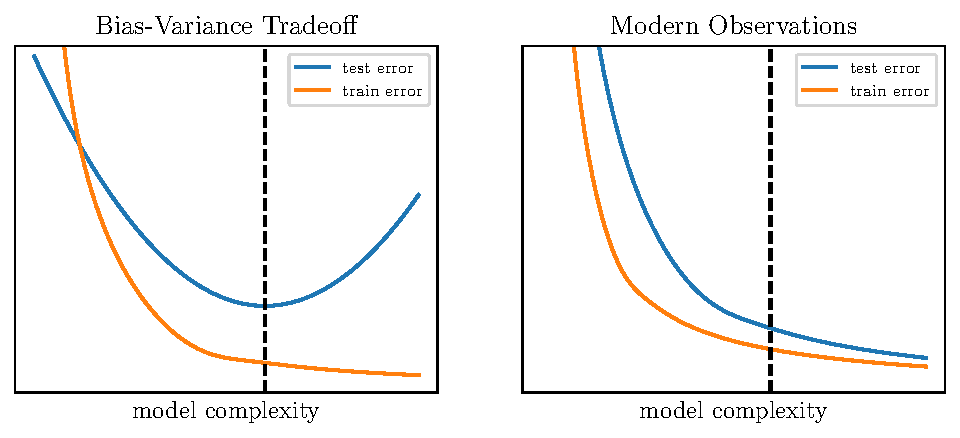
\includegraphics[width=0.8\textwidth, height=0.2\textheight]{old_new.pdf}
		\caption{Common wisdom and many empirical observations suggest that the training error decreases with the complexity of the hypothesis class. The test error decreases as well, only to increase again after a certain threshold as shown in the figure on the left. Here, the threshold usually corresponds to the point where the number of learnable parameters equals the size of the dataset. However, modern observations suggest that deep neural networks can have many parameters and still generalize well as shown in the figure on the right.}
\end{figure}
Recently, there has been a lot of research to understand the phenomenon of
overparameterization. While we will not delve into the details of this research,
we look at a one specific example. 
\begin{boxedexample}
	\label{ex:generalization}
	Consider as a hypothesis class the space of 2-layer neural networks with ReLU
	activation functions. Assume that the learnable weights
	corresponding to the first layer do not deviate much in the 2-norm from
	their initial values. Further, assume that the weights of the second layer
	remain bounded in the 2-norm throughout the training. Formally, this class can be written as
	$$
		\mathfrak{H} := \{h(x) = V \cdot [U\cdot x]_+: U, V \in W\},
		$$
		where
		\begin{align*}
		W :=& \{(U,V) \quad U \in \mathbb{R}^{n \times n_{\text{hu}}}, V \in \mathbb{R}^{n_\text{hu} \times n_{\text{class}}} \quad \text{and}\\
		& \quad \|u_i-u_i^0\|_2 \leq \beta, \|v_i\|_2 \leq \alpha \quad \text{for all units}\}, 
		\end{align*}
		and $n_\text{hu}$ is the number of hidden units, $n_{\text{class}}$ is the
		number of classes, $[.]_+$ denotes the ReLU activation function, $u_i$,
		$v_i$ denote the $i$-th column of $U$ and $V$, respectively, $u_i^0$, $v_i^0$ are the $i$-th column of the
		initial weight matrix $U$, and $V$, respectively, and $\beta$ and $\alpha$ are
		constants.		

		Train such a neural network on the publicly available CIFAR-10 dataset.
		Study empirically both the training error and the test error as a
		function of the number of hidden units. What do you observe? Experiment
		with $n_{\text{hu}}$ ranging from 8 to 30000. 

		Now, empirically study the quantities $\|U\|_2$, $\|V\|_2$, and
		$\|U-U^0\|_2$ as a function of the number of hidden units. What do you observe?
\end{boxedexample}

In \cite{Neyshabur:arXiv1805} the authors did the empirical study explained in
\Cref{ex:generalization} and observed the following:
\begin{itemize}
	\item Both the training error and test error decrease as a function of
	$n_{\text{hu}}$. This indicates that we are in the overparameterization
	regime.
	\item The quantity $\|U\|_2$ initially decreases as a function of
	$n_{\text{hu}}$ and then increases. The quantities $\|V\|_2$ and
	$\|U-U^0\|_2$ decrease as a function of $n_{\text{hu}}$. 
\end{itemize}
The second observation, and specifically the decrease of $\|U-U^0\|_2$ as a
function of $n_{\text{hu}}$, is particularly interesting. It suggests that the
weights of the neural network do not deviate much from their initial values
during training. It appears here that training the neural network is then more
focused on optimizing the weights of the second layer. When interpreting the
hidden units as features, this result suggests that when one has many features,
one has consequently many relevant features that are useful for the task at
hand. Hence, there is no need to learn new features. 

In a next step, the authors bounded the Rademacher complexity of the specific
hypothesis class in \Cref{ex:generalization} by the quantities $\|U-U^0\|_2$ and
$\|V\|_2$. In particular, they showed that
$$
\text{Rad}(l \circ \mathfrak{H} \circ D) \leq \frac{C}{\sqrt{m}} \max_i \|x_i\|_2 \ \alpha \ (\beta+ \|U^0\|_2)
$$

This suggests that the Rademacher complexity of the
hypothesis class decreases as a function of $n_{\text{hu}}$, which is in
line with the empirical observations.

\section*{Wait! What is what?}
Here is a list of questions that help you check your understanding of key
concepts inside this chapter.

\begin{enumerate}
    \item What is the ultimate goal of a supervised learning problem? 
    \item  Where does the randomness in probably-approximately-correct (PAC) learning come from?
    \item What is the realizability assumption in PAC learning?
    \item What is the empirical risk minimization principle?
    \item How do we judge whether a certain type of a complexity measure of a hypothesis class is good?
    \item What is the bias-variance tradeoff? How does it relate to the complexity of the hypothesis class?
    \item What are the limitations of the VC-dimension as a complexity measure of a hypothesis class?
    \item What is the overparameterization regime?
\end{enumerate}


% Chapter 1
% !TeX spellcheck = en_US 
\chapter{Neural networks} % Main chapter title

\label{Chapter3} % For referencing the chapter elsewhere, use \ref{Chapter1} 
\setcounter{chapter}{3}
%\setcounter{section}{0}
In the \nameref{Chapter1} chapter, we breifly talked about a neural network which can be used 
to recognize hand-written digits. The neural network takes an image of a hand-written digit as 
an input and predicts a number which corresponds to the digit as an output. In this chapter, 
we will delve deeper into the architecture of neural networks and try to answer the following questions:
\begin{enumerate}
    \item What is the motivation behind using neural networks ?
    \item What is the idea behind the structure (neurons, input layer, hidden layers, output layer) 
    of neural networks ?
    \item Why do we need an activation function and a loss function ?
    \item How to train a neural network ?
    \item What are learning algorithms ?
    \item Why certain neural networks can approximate any continuous function defined on a compact set ?
\end{enumerate}
Recognition of handwritten digits is a classic problem for introducing the topic of neural networks. Therefore 
we will use this problem as an example to introduce various concepts related to neural networks.
  
%%%%%%%%%%%%%%%% Handwritten digit recog %%%%%%%%%
\section{Handwritten digit recognition}
Most people can easily recognize the handwritten digits shown in figure \ref{fig:my_digits}. Even if these digits were written 
in a different manner (for example refer figure \ref{fig:my_threes} ), one would still be able to recognize them. 
\begin{figure}[htbp]
    \centering
    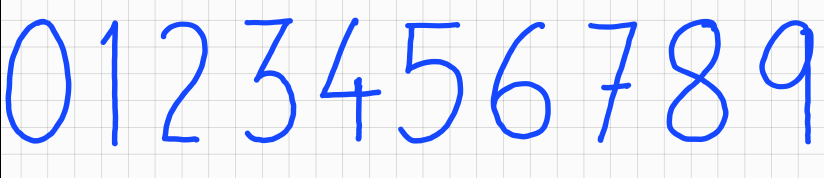
\includegraphics[width=.6\textwidth]{Figures/digits.png}
    \caption{One of the ways of writing digits from $1$ to $9$.}
    \label{fig:my_digits}
\end{figure} 
\begin{figure}[htbp]
    \centering
    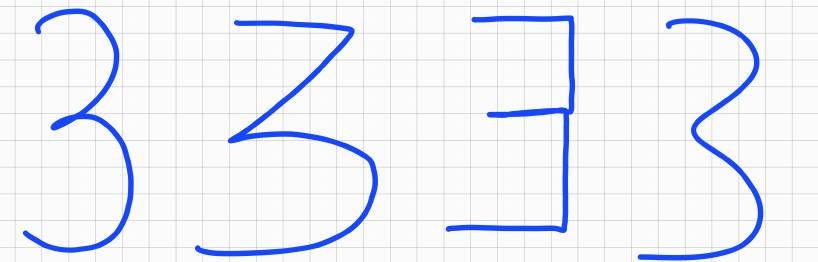
\includegraphics[width=.3\textwidth]{Figures/three_digit.png}
    \caption{Different ways of writing the digit $3$.}
    \label{fig:my_threes}
\end{figure} This is due to the fact that our visual cortex has evolved over millions of years and therefore is magnificently 
adapted to understand the visual world \cite{vis_cortex}. The problem of recognizing hand-written digits is so trivial 
for our brains that we don't have to put an effort to recognize digits. But this task will immediately 
start to look complicated when one tries to write a computer program which can recognize hand-wriiten 
digits. 
Let us try to write a program for this task. We can start by coverting the digits into a pixel 
image ($28 \times 28$ for example) and assigning each pixel a value from $0$ to $1$ based upon the level of 
darkness/brightness (figure \ref{fig:pix7}). This can serve as an input to our program. 
\begin{figure}[htbp]
    \centering
    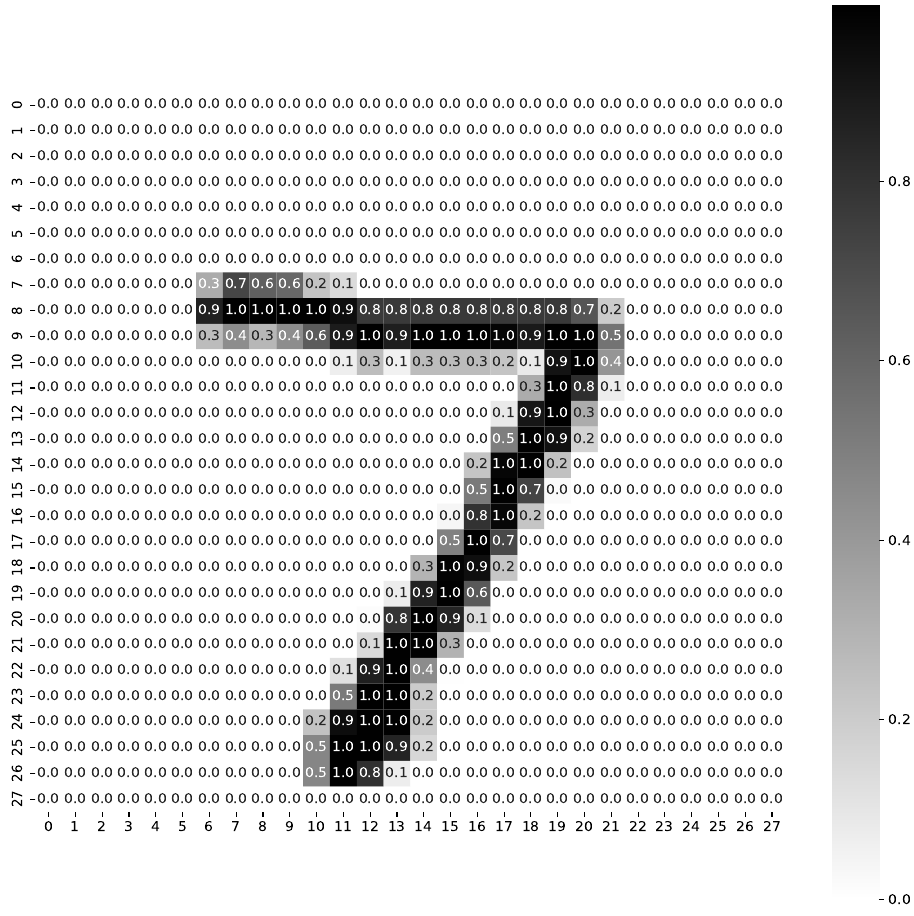
\includegraphics[width=.35\textwidth]{Figures/pixel_image_7.png}
    \caption{A $28 \times 28$ pixel image of digit $7$. Each pixel is assigned a value from $0$ to $1$.}
    \label{fig:pix7}
\end{figure} 
We can identify distinct features of each digit and write code which looks for these features in the input image. 
Our program will therefore contain a lot of \emph{if} statements and \emph{for} loops to identify such features 
but more importantly will contain thousands of line of code to handle exceptions which arise from the fact that 
each digit can be written in a slightly different manner. It turns out that it is very difficult to express algorithmically 
the intuitions we have for recognizing digits. Soon we will realize the complexity of this task. What if we could write a 
program (for such fuzzy and difficult to-reason-about problems) that mimics the structure of our brain ?  
%%%%%%%%%%%%%%%% Intro to NN %%%%%%%%%%%%%
\section{Introduction to neural networks}
Neural networks tackles this problem in a different way. The construction of neural network
is inspired by the structure of our brain. 
\begin{figure}[htbp]
    \centering
    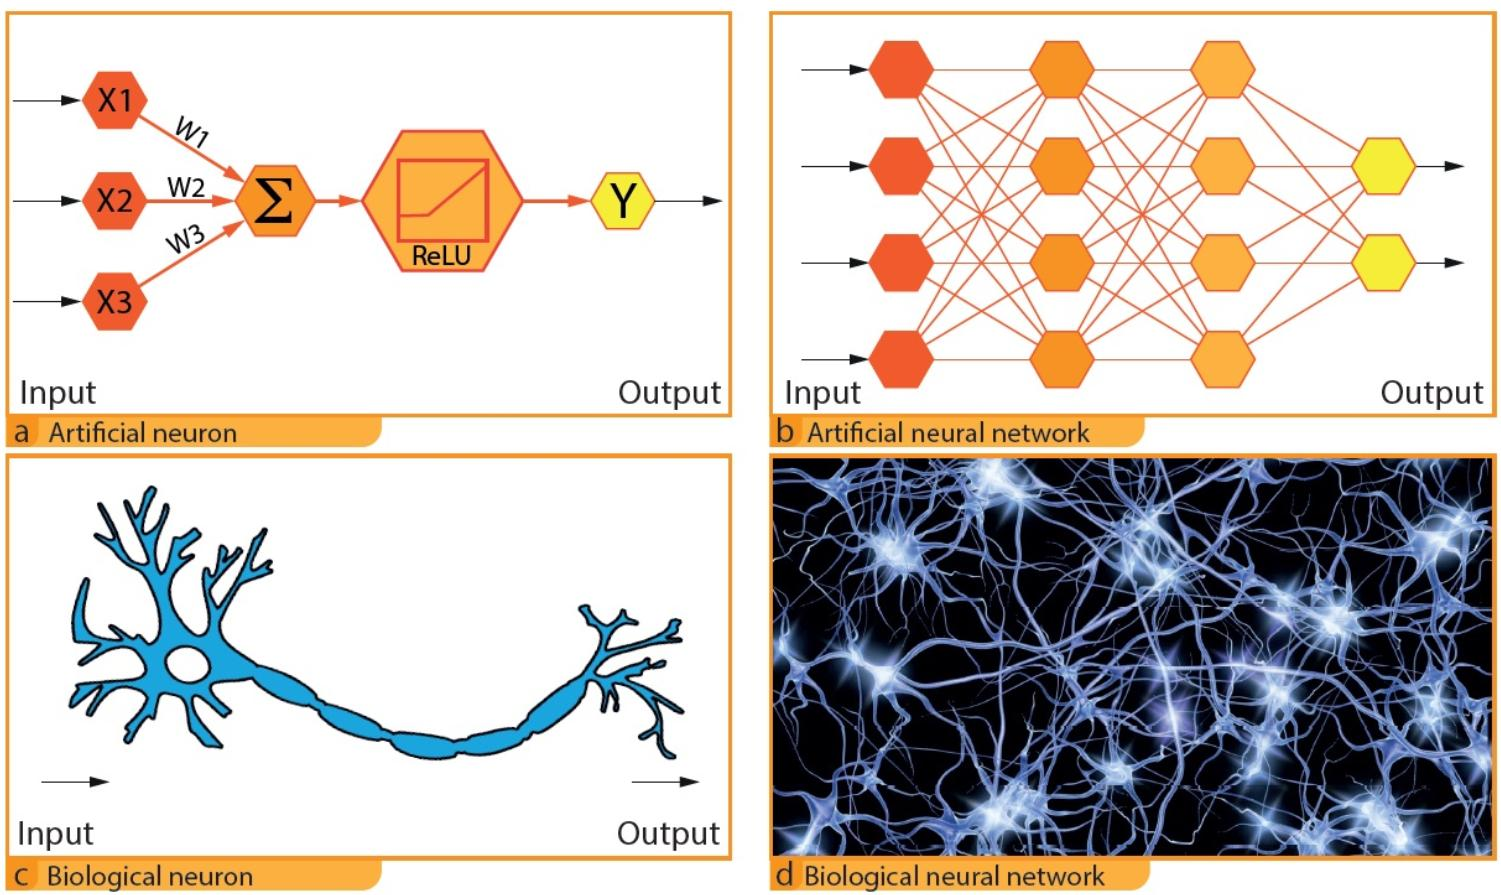
\includegraphics[width=.5\textwidth]{Figures/artificial_vs_normal_neurons.png}
    \caption{Similarity between the structure of artificial and biological neuron \cite{bio_art_neuron}.}
    \label{fig:bio_neu}
\end{figure} 
The idea is to take a large number of handwritten digits together with labels and develop a system 
which can learn from these examples just like we learn. We leave it to the system to automatically infer rules 
from these examples and classify hand-written digits. 
\begin{figure}[htbp]
    \centering
    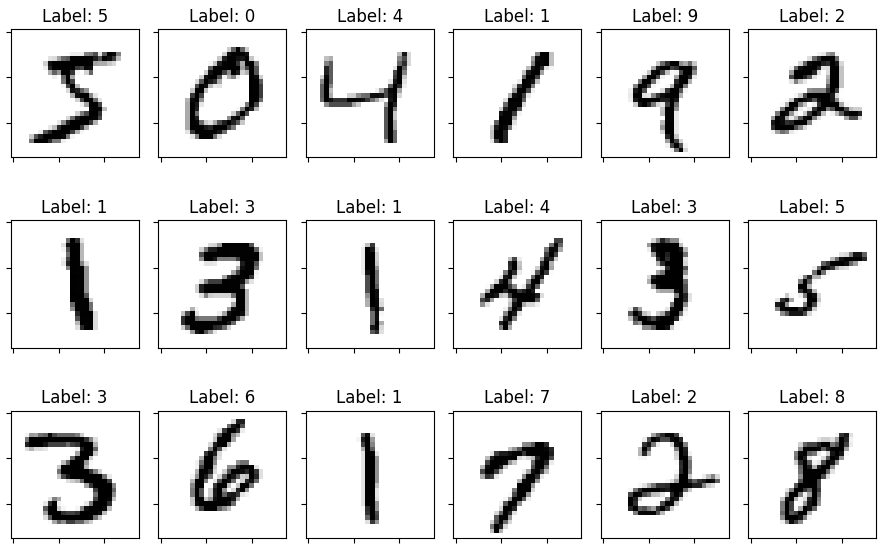
\includegraphics[width=.5\textwidth]{Figures/training_examples_mnist.png}
    \caption{Some training examples from MNIST dataset \cite{lecun1998mnist}.}
    \label{fig:train_MNIST}
\end{figure} 

A neural network takes an input and gives an output. Figure \ref{fig:ff_net} shows a pictorial representation of
a neural network which can be used to classify handwritten digits. It has layers (input, hidden, output) which consist of 
artificial neurons. The neurons are connected. Each neuron stores a value (for example from $0$ to $1$ in 
our case of handwritten digit recognition). 
\begin{figure}[htbp]
    \centering
    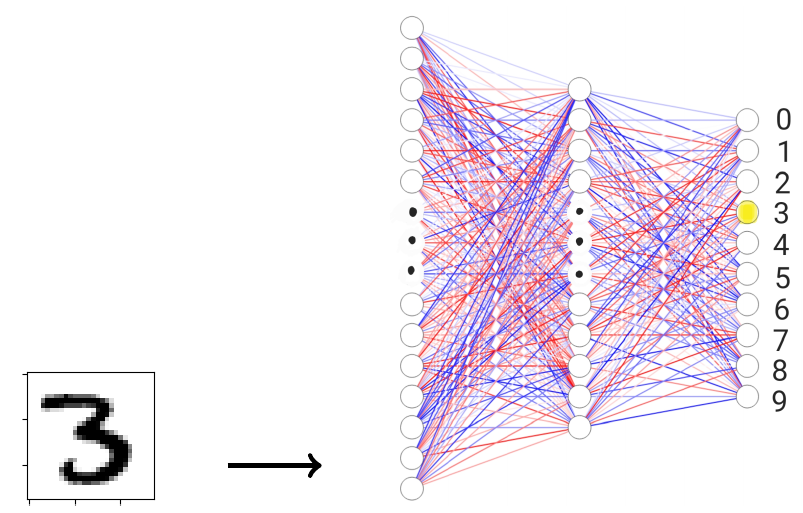
\includegraphics[width=.8\textwidth]{Figures/ff_net.png}
    \caption{A neural network to classify handwritten digits \cite{nn_SVG}.}
    \label{fig:ff_net}
\end{figure} 
A neuron takes multiple inputs (say $a_1, a_2,....,a_n$) and gives the output $\sigma(\sum_{i =1}^n a_i w_i + b)$ where $\sigma$ is
called an activation function. The inputs are multiplied by weights, $w_i$ and added to a bias, $b$ before passing through the activation funciton.
The choice of activation function depends on the type of problem one is trying to solve. For example, for hand-written digit recognition one could use sigmoid/logistic function
as an activation function. 
\begin{figure}[htbp]
    \centering
    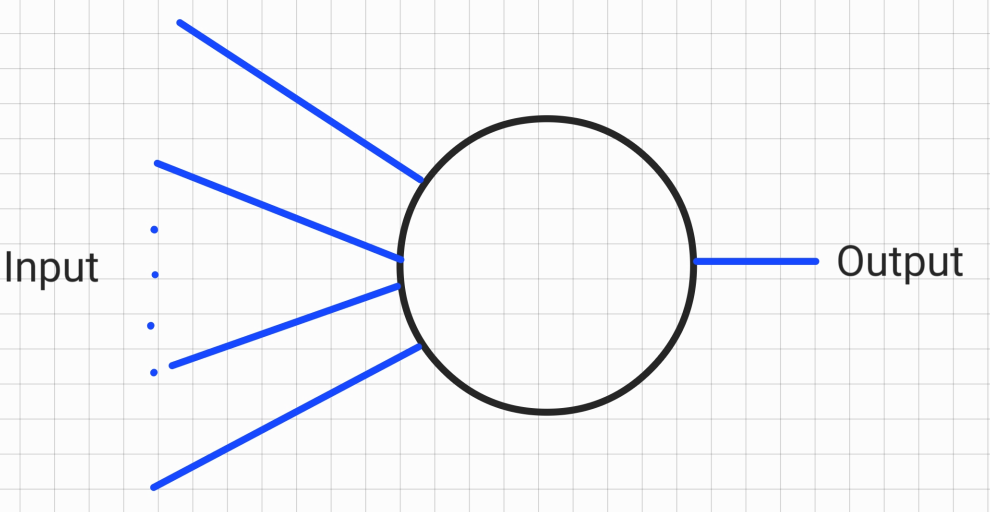
\includegraphics[width=.4\textwidth]{Figures/neuron.png}
    \caption{A pictorial representation of an artificial neuron. It takes 
    multiple inputs (say $a_1, a_2,....,a_n$) and gives the output $\sigma(\sum_{i =1}^n a_i w_i + b)$.}
    \label{fig:neuron}
\end{figure} 
\begin{figure}[htbp]
    \centering
    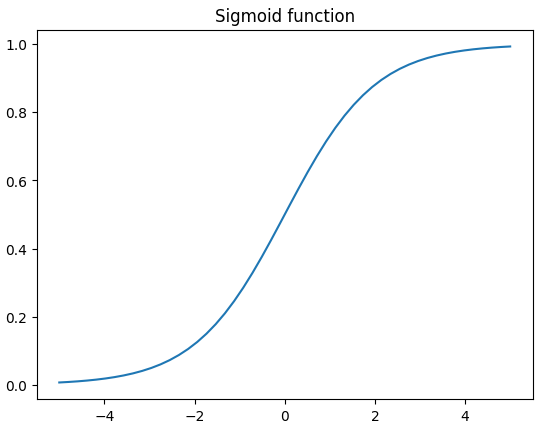
\includegraphics[width=.4\textwidth]{Figures/sigmoid.png}
    \caption{A sigmoid/logistic activation function, $\sigma (z) = \frac{1}{1+ e^{-z}}$}
    \label{fig:sig}
\end{figure} 

Mathematically speaking, a neural network is simply a function that takes an input which passes through
its layers (made up of neurons which are mathematical functions) and results in an output. The neural 
network shown in figure \ref{fig:ff_net} has $784$ neurons in the input layer (containing data from a $28 \times 28$ pixel image), $15$
neurons in the hidden layer and $10$ neurons in the output layer. Each neuron in the output layer corresponds to a digit from $0$ to $9$; if
the input image is of digit $3$, only the fourth neuron in the outplayer will light up (output is close to $1$) while the rest will remain dormant (outputs are closer to $0$).
Such neural networks are called feed-forward neural networks. When we look at the architecture of a neural network, many questions can 
come to our minds, for example, 
\begin{enumerate}
    \item Why does the network has a particular structure (i.e. layers with neurons) ?
    \item What is the purpose of using an activation function ?
    \item How does a neural network able to recognize hand-written digits ?
\end{enumerate} 
Until now, it is also not clear that why this approach (of using neural networks) even works. Even if we assume that this approach works, another question arises,
which is, how do we get the weights, $w_i$ and biases $b_i$ of the network ? The answer to this question
comes from a key ability of neural networks which is \emph{learning}.
%%%%%%%%%%%%%%%% Learning from data %%%%%%%%%%%
\subsection{Learning from data}
Learning is the process of obtaining suitable weights and biases such that a neural network can perform
the desired task. There are several steps involved in learning. First step is to assign random values to 
weights and biases of the network and show the network some training examples. In the case of handwritten digit recognition
we use the MNIST dataset \cite{lecun1998mnist}. Since the network is initialized with random weights and biases it will wrongly classify handwritten digits. 
\begin{figure}[htbp]
    \centering
    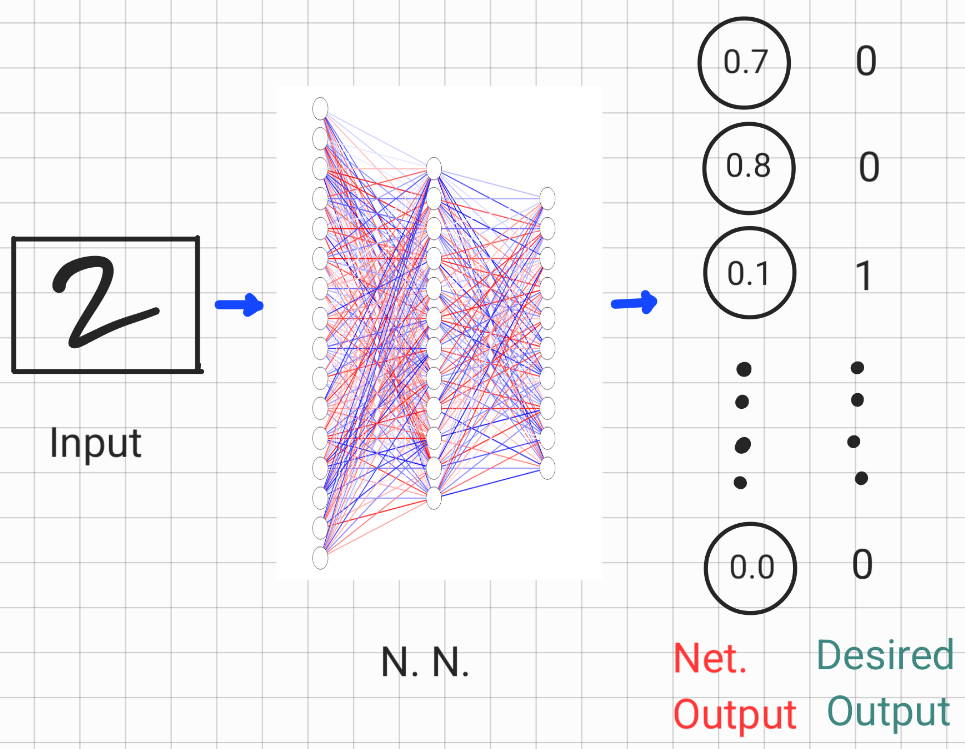
\includegraphics[width=.4\textwidth]{Figures/rand_inp.png}
    \caption{Results from a randomaly initialized neural network and how it compares to the desired output for a training example}
    \label{fig:randinp}
\end{figure} 
Next step is to tell the network to update its weights and biases in order to reduce the classfication error. This is done by introducing a 
cost/loss function which can quantify the classification error. We use a quadratic loss function, 
$$C(w,b) = \frac{1}{N} \sum_x {\|y(x) - a\|}^2$$
where $N$ denotes the number of training examples, $y(x)$ is the desired output corresponding to training example $x$, and 
$a$ is the neural network output. Our aim is to find $w,b$ such that the loss is minimum. The problem of learning from training data thus translates into
solving an optimization problem. But this process raises another set of questions,
\begin{enumerate}
    \item Which optimization algorithm to choose for minimizing the cost function?
    \item How to define a suitable loss function ?
    \item Does a global minimum exists for a chosen loss function ?
\end{enumerate}
To answer these questions and the questions that we raised earlier, we will have to first understand the origins of neural networks.
%%%%%%%%%%%%%% Origins of NN %%%%%%%%%%%%%%
\subsection{Origins of neural networks}
The artificial neurons we introduced earlier are called sigmoid neurons. In order to understand 
why sigmoid neurons are defined the way they are, we need to first understand another artificial 
neuron called perceptron. Perceptrons were developed in the $1950$s and $1960$s \cite{rosenblatt1958perceptron}. Unlike sigmoid neurons 
whose inputs, $x_i \in \mathbb{R}$, a perceptrons can take only binary inputs and produce a binary output.
The mathematical model of a perceptron is,
\begin{equation*}
    \text{output} = 
     \begin{cases}
       0 &\quad \text{if} \ \ \sum_i w_i x_i \leq \ \text{threshold} \\
       1 &\quad  \text{if} \ \ \sum_i w_i x_i > \ \text{threshold} 
     \end{cases}
\end{equation*}
where $x_i$ are the inputs and $w_i$ are the weights. The output is $1$ if $\sum_i w_i x_i$ exceeds a threshold 
value otherwise the output is $0$. Perceptrons can be used as a device to make simple decisions by weighing up evidence \cite{nielsen2015neural}. 
The following example illustrates how perceptrons can be used to make a decision.
\begin{boxedexample}
    Suppose a Rock band is coming to perform in your city. You like Rock music and you are trying to 
    decide whether or not to go to this event. You can make the decision by weighing up three factors:
   \begin{enumerate}
    \item Is the event nearby ?
    \item Are your friends accompanying you ?
    \item Is the weather good ?
   \end{enumerate}
   We can assign binary variables $x_1, x_2$ and $x_3$ to these three factors. For example, if the event is nearby we would
   have $x_1 =1$ but if it is far away we would have $x_1 = 0$. Similarly, if your friends are accompanying you, $x_2 =1$ otherwise $x_2 =0$.
   If the weather is good, $x_3 =1$ and if the weather is bad, $x_3 =0$. Now suppose, you absolutely love rock music and it doesn't really 
   matter to you if your friends can accompany you or if the event is nearby but you really loathe bad weather and you won't go if the
   weather is bad. You can use perceptrons to model this kind of decision-making. One way is to choose, $w_3 = 6$ for the weather and
   $w_1 =2, w_2 =2$ for other conditions. The larger value of $w_3$ in comparison to $w_1$ and $w_2$ suggests that weather matters to you a lot. 
   Finally, suppose you choose a thresold value of $5$ for the perceptron. With these choices, the perceptron mimics the desired 
   decision-making model, outputting $1$ whenever the weather is good, and $0$ whenever the weather is bad. By choosing different values for 
   weights and the thresold, we can get different models of decision making. 
\end{boxedexample}
It is obvious that the perceptron isn't a complete model of human descision-making. But it is plausible that if we use more layers in the network
with more number of perceptrons, the network could make more complex decisions:
\begin{figure}[htbp]
    \centering
    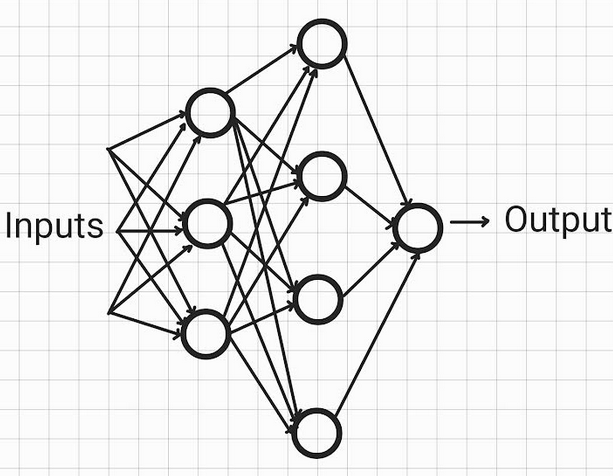
\includegraphics[width=.4\textwidth]{Figures/perceptron_network.png}
    \caption{A network built out of perceptrons.}
    \label{fig:percep_net}
\end{figure} 
We can write the mathematical model of a perceptron in a way familiar to us, 
\begin{equation*}
    \text{output} = 
     \begin{cases}
       0 &\quad \text{if} \ \ \sum_i w_i x_i + b \leq 0 \\
       1 &\quad  \text{if} \ \ \sum_i w_i x_i + b > 0 
     \end{cases}
\end{equation*}
where perceptron's bias, $b \equiv -$threshold. We have seen that a network of perceptrons can be used as 
a method for weighing evidence to make decisions. We can also use perceptrons to compute the elementary logical functions such as
AND, OR, and NAND \cite{nielsen2015neural}. The NAND gates are universal for computation, and therefore it follows that perceptrons are also universal for
computation \cite{nielsen2015neural}. This property of perceptrons tells us that networks of perceptrons can be as powerful as any other computing device. These 
properties of perceptrons might make them an attractive option for solving decision-making problems but the property that we 
are really looking for in the network is the ability to tune its weights and biases in response to external stimuli (for example training data).
We want our network to learn from data. In order to devise learning algorithms for a network, we would like that if we make 
a small change in some weight (or bias) in the network, the output changes only by a small amount. Schematically, this is what we want:
\begin{figure}[htbp]
    \centering
    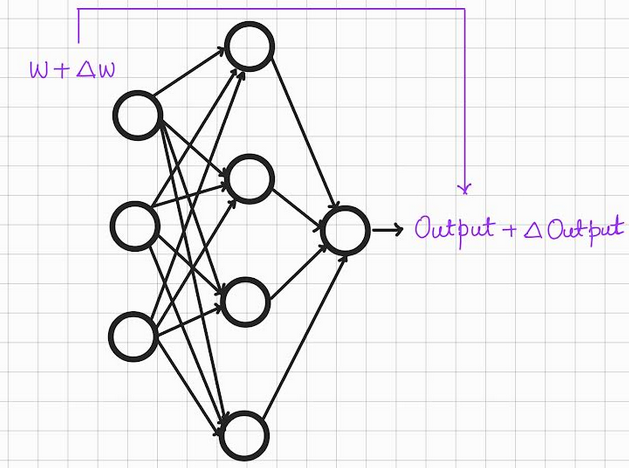
\includegraphics[width=.4\textwidth]{Figures/precepnet2.png}
\end{figure}
 
Unfortunately, a network of perceptrons doesn't have this capability. This is the reason why we use sigmoid neurons. Unlike perceptrons, the sigmoid 
neurons can take input values between $0$ and $1$. The activation function used in sigmoid neurons can be described as, 
$$\sigma(z) = \frac{1}{1 + e^{-z}}.$$
The smoothness of $\sigma$ ensures that a small change in the input causes a small change in the output. 

Figure \ref{fig:deepNN} shows an architecture of a typical (feed-forward) neural network. It consists of an input layer, multiple hidden layers and an output layer. The choice of
the number of neurons in the input and output layers is governed by the problem one is trying to solve. For example, in the case of 
hand-wriiten digit recognition, if the input image consists of data from $28 \times 28 = 784$ pixels, the input layer will have $784$ neurons. We want to classify the 
images into digits from $0$ to $9$ and therefore the output layer will have $10$ neurons. The design (number of layers and number of neurons) of hidden layers
is based on heuristics. Let us now look at a neural network (in detail) which can classify handwritten digits. 
\begin{figure}[htbp]
    \centering
    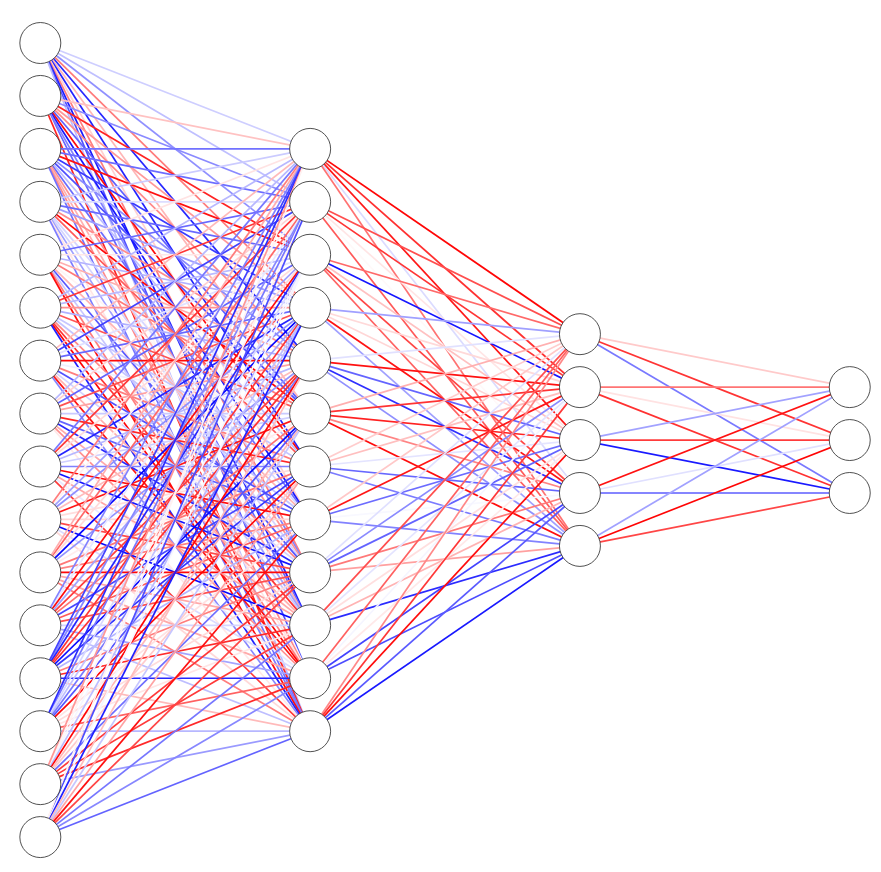
\includegraphics[width=.4\textwidth]{Figures/DeepNN.png}
    \caption{A feedforward neural network with an input layer $\in \mathbb{R}^{16}$, two hidden layers and an output layer $\in \mathbb{R}^2$ \cite{nn_SVG}.}
    \label{fig:deepNN}
\end{figure}
%%%%%%%%%%%% network to classify HD %%%%%%%%%%%%
\subsection{A network to classify handwritten digits}
We use a network consisting of an input layer $\in \mathbb{R}^{784}$, one hidden layer and an output layer $\in \mathbb{R}^{10}$ to classify handwritten
digits (see figure \ref{fig:NN_HD}). Let us try to understand how this neural network works. 
\begin{figure}[htbp]
    \centering
    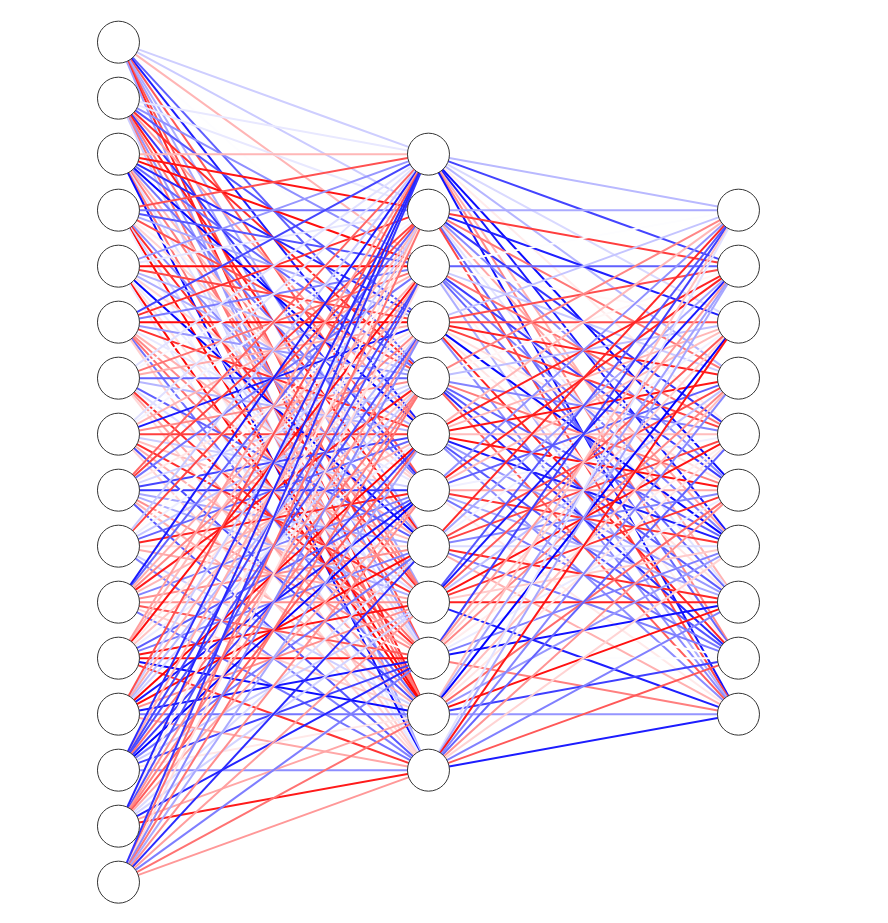
\includegraphics[width=.4\textwidth]{Figures/NN_2.png}
    \caption{A pictorial represenation of a neural network which can classify handwritten digits. It consists of an input layer $\in \mathbb{R}^{784}$ (only a few neurons are shown in the figure), one hidden layer and an output layer $\in \mathbb{R}^{10}$.}
    \label{fig:NN_HD}
\end{figure} 
The main feature of this network is its ability to learn from data. We use MNIST data set which consists of scanned images of digits written by $250$ people \cite{lecun1998mnist}. The MNIST data
comes in two parts; a training data set containing $60000$ imgaes and a test data set containing $10000$ images. The images are in grescale and have size of $28 \times 28$ pixels.
The MNIST data, along with hand-written digits, also provide correct labels corresponding to the digits. 
\begin{figure}[htbp]
    \centering
    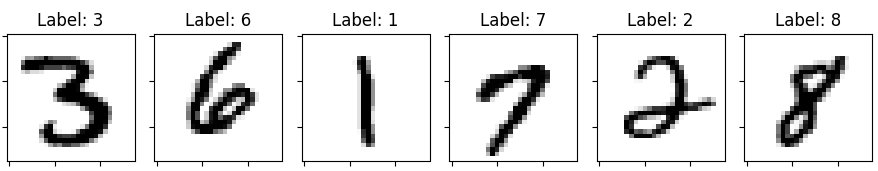
\includegraphics[width=.4\textwidth]{Figures/mnist_data_sample.png}
    \caption{A sample of training data from MNIST data set.}
    \label{fig:mnist_data}
\end{figure} 
The input $x$ to the network is a $28 \times 28 = 784$ dimensional vector and the output $a$ is a $10$ dimensional vector. In order to quantify, the 
accuracy of this network's prediction, we define a cost/loss function,
$$C(w,b) = \frac{1}{N} \sum_x {\|y(x) - a\|}^2$$
where $N$ denotes the number of training examples, $y(x)$ is the desired output (a $10$ dimensional vector) corresponding to a training example $x$, and 
$a$ is the neural network output. The idea is to find weights and biases which minimizes the difference between the desired output (labels) and the network prediction and we want this to happen for all training examples. For example, 
if an input $x$ is an image of digit $6$, we want our network's output $a$ to be as close as possible to $y(x) = (0,0,0,0,0,0,1,0,0,0)^T$. The problem of 
minimizing the loss function is an optimization problem. In the context of neural networks, the most popular methods which are used to minimize the loss function are 
inspired from the gradient descent method. 

Let us consider a simple example to understand the gradient descent method. Suppose we want to minimize a function $C(\mathbf{v})$ of two variables $v_1$ and $v_2$ (see figure \ref{fig:cost_f}).
\begin{figure}[htbp]
    \centering
    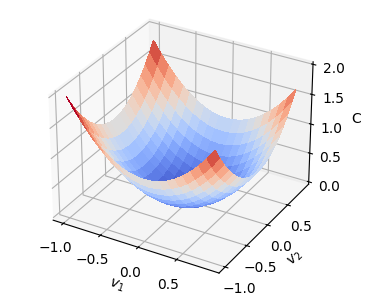
\includegraphics[width=.4\textwidth]{Figures/cost_func.png}
    \caption{A function $C$ of two variables $v_1$ and $v_2$.}
    \label{fig:cost_f}
\end{figure} 
We can use Calculus to calculate the gradients of $C(\mathbf{v})$ with resprect to $v_1, v_2$ and use them to find places where $C$ is minimum. This method could work well when 
$C$ is a function of few variables but soon will turn into a nightmare when we increase the number of variables. Typically, the cost function of a neural network depends on a large number of
weights and biases; in fact the biggest neural networks consists of billions of weigths and biases. Therefore, one has to come up with cost effective 
methods of finding the minima of cost functions. Grandient descent is one such method. It is an interative method, where one starts 
with an initial guess for variables and update them over multiple iterations in such a 
way that the cost function reduces with each iteration. Consider the case of cost function $C(\mathbf{v}$). For small changes $\Delta v_1$ and  $\Delta v_2$ in variables $v_1$ and 
$v_2$ respectively, we can write the change in cost function $\Delta C$ as
\begin{equation}
    \label{eq:del_C}
    \Delta C \approx \frac{\partial C}{\partial v_1}\Delta v_1 + \frac{\partial C}{\partial v_2} \Delta v_2 = \nabla C \cdot \Delta \mathbf{v}
\end{equation}
The aim is to find suitable change $\Delta \mathbf{v}$ which leads to reduction in $C$ i.e. $\Delta C < 0$. One such choice is $\Delta \mathbf{v} = -\eta \nabla C$ provided $\eta > 0$,
$$\Delta C \approx \nabla C \cdot \eta \nabla C = \eta \|\nabla C\|^2 < 0 $$
To conclude, in the gradient descent method we start with an initial guess $\mathbf{v}$ and update it by following
 $$\mathbf{v} \rightarrow \mathbf{v}' = \mathbf{v} - \eta \nabla C$$
untill we reach the minimum of $C(\mathbf{v})$. In the context of neural networks, a gradient descent update might look like this, 
\begin{equation}
    \begin{aligned}
        w_j \rightarrow w_j' = w_j - \eta \frac{\partial C}{\partial w_j}\\
        b_k \rightarrow b_k' = b_k - \eta \frac{\partial C}{\partial b_k}.
    \end{aligned}
\end{equation}
Note that the parameter $\eta$ should be sufficiently small in order to justify the assumption in equation \eqref{eq:del_C}. 
We call this parameter the \emph{learning rate}. The use of gradient descent method might seem as a
good alternative to using analytical methods but there are still a number of challenges in applying this method. Notice that the cost function has the form
$C = \frac{1}{N} \sum_x C_x$, that is, it's an average overs costs $C_x = \|y(x) - a\|^2$ for individual training examples. In order to make an update of gradient
descent, we need to compute the gradients $\nabla C_x$ separately for each training input and then average them, $\nabla C = \frac{1}{N} \sum_x \nabla C_x$. This update can take 
extremely long time to make when the number of training inputs are very large, thus making the \emph{learning} very slow. 

We can overcome the issue of slow \emph{learning} by using a variant of gradient descent method called \emph{stochastic gradient descent (SGD)} method. The idea is to estimate the gradient
$\nabla C$ by computing $\nabla C_x$ for a small sample of training examples and use it to make updates in weights and biases. The following steps are involved in using the stochastic gradient descent method,
\begin{enumerate}
    \item Shuffle the training inputs and divide into batches of size $m$. Each batch (we call them mini-batches) consists of training examples say, $X_1, X_2, .....X_m$.
    \item Calculate gradients for one mini-batch: $$\frac{1}{m} \sum_{i=1}^{m} \nabla C_{X_i} \approx \frac{1}{N} \sum_x \nabla C_x = \nabla C$$
    \item Make an update in the weights and biases: 
    $$w_j \rightarrow w_j' = w_j - \frac{\eta}{m} \sum_i \frac{\partial C_{X_i}}{\partial w_j}$$
    $$b_k \rightarrow b_k' = b_k - \frac{\eta}{m} \sum_i \frac{\partial C_{X_i}}{\partial b_k}$$
    \item Pick another mini-batch from the shuffled data and repeat steps $2$ and $3$ until all training inputs are exhausted. The end of this step is referred to as an \emph{epoch} of training.
    \item Repeat steps $1$ to $5$ until the network is sufficiently trained.
\end{enumerate}
The use of SGD significantly increases the speed at which a network is trained. We may be making less accurate updates (hence the name \emph{stochastic}) in the weights and biases in comparison to 
standard gradient descent method but nevertheless the updates are faster and over multiple iterations the cost (on an average) does go down. 
\section{Backpropagation}
Backpropagation is a fast algorithm for computing gradients \cite{nielsen2015neural}. Today, it is the workhorse of learning in neural networks. It uses chain-rule from 
Calculus to compute gradients $\frac{\partial C}{\partial w_i}, \frac{\partial C}{\partial b_i}$ and in the process reveals how changing the weights and 
biases changes the overall behaviour of the network. We will first see how backpropagation works for a very simple neural network and then generalize the procedure for
big neural networks \cite{backprop_grant}. Consider a neural network having one neuron in the input layer, two hidden layers each with one neuron and one neuron in the output layer (see figure \ref{fig:sim_NN}). 
\begin{figure}[htbp]
    \centering
    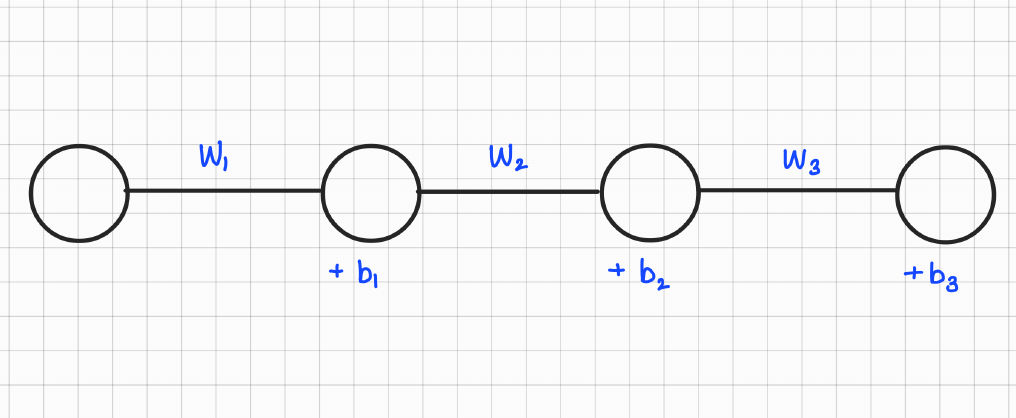
\includegraphics[width=.5\textwidth]{Figures/simpNN.png}
    \caption{A simple neural network with only neuron in each layer}
    \label{fig:sim_NN}
\end{figure} 
We can write the loss function as 
$$C = \frac{1}{N} \sum_{k=0}^{N-1} C_k.$$
Let us focus on the cost correponding to one training example,
$$C_0 = (a^{(L)} - y)^2$$ 
where $a^{(L)}$ is the network output and $y$ is the desired output. We label the activation/output from the last neuron with a superscript $L$, indicating which layer it's in, so the
activation of the previous neuron becomes $a^{(L-1)}$. We can express the last activation $a^{(L)}$ by 
$$a^{(L)} = \sigma (w^{(L)}a^{(L-1)} + b^{(L)})$$
where $w^{(L)}$ and $b^{(L)}$ denote the weight and bias of the last neuron respectively. We introduce a new variable $z$ (called weighted sum) for the input to the activation function and keep the same superscript as the activation for labeling it:
$$z^{(L)} = w^{(L)} a^{(L-1)} + b^{(L)}$$
$$a^{(L)} = \sigma (z^{(L)}) $$
We first calculate $\frac{\partial C_0}{\partial w^{(L)}}$ which gives us a measure of how changes in $w^{(L)}$ affects $C_0$. We use the chain-rule from Calculus and write, 
\begin{equation}
    \label{eq:sim_grad_w}
    \frac{\partial C_0}{\partial w^{(L)}} = \frac{\partial z^{(L)}}{\partial w^{(L)}} \frac{\partial a^{(L)}}{\partial z^{(L)}} \frac{\partial C_0}{\partial a^{(L)}}
\end{equation}
The terms in equation \eqref{eq:sim_grad_w} become clear if we refer to the tree of variables of the network (figure \ref{fig:tree_NN}). We can express the terms in equation \eqref{eq:sim_grad_w} by
\begin{equation*}
    \begin{aligned}
        & \frac{\partial z^{(L)}}{w^{(L)}} = a^{(L-1)} \quad \text{since} \ z^{(L)} = w^{(L)} a^{(L-1)} + b^{(L)}\\
        & \frac{\partial a^{(L)}}{\partial z^{(L)}} = \sigma'(z^{(L)}) \quad \text{since} \ a^{(L)} = \sigma (z^{(L)})\\
        & \frac{\partial C_0}{\partial a^{(L)}} = 2 (a^{(L)} - y) \quad \text{since} \ C_0 = (a^{(L)} - y)^2.
    \end{aligned}
\end{equation*}
where $\sigma'(z^{(L)})$ denotes the derivative of the activation function. This reduces equation \eqref{eq:sim_grad_w} to 
\begin{equation}
    \label{eq:del_w}
    \frac{\partial C_0}{\partial w^{(L)}} = a^{(L-1)} \cdot \sigma'(z^{(L)}) \cdot 2(a^{(L)} -y). 
\end{equation}
\begin{figure}[htbp]
    \centering
        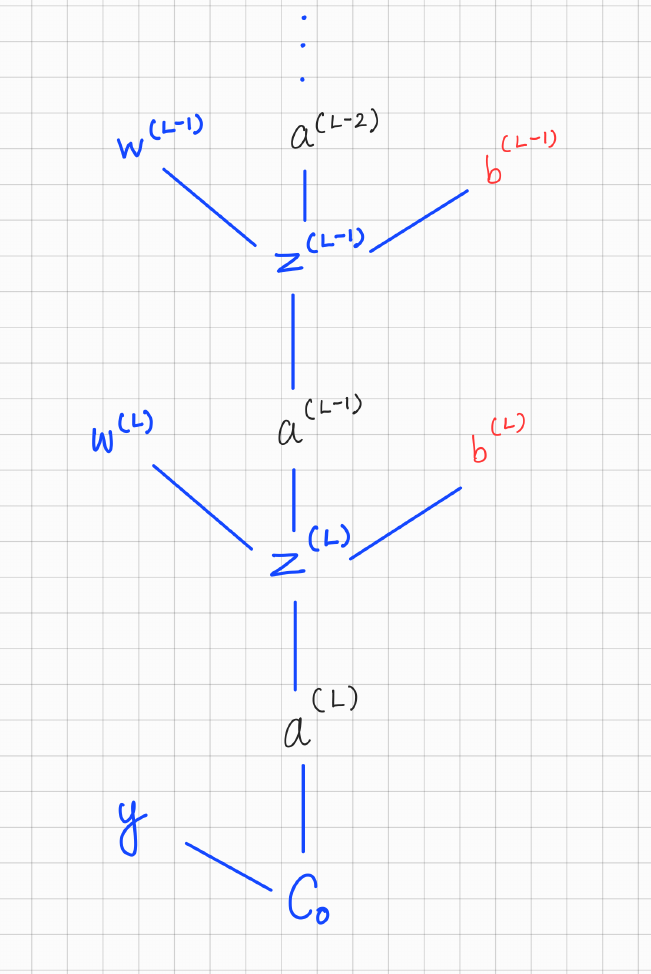
\includegraphics[width=.5\textwidth]{Figures/treeNN.png}
        \caption{This tree shows how the variables are connected in the neural network}
        \label{fig:tree_NN}
    \end{figure} 
Next, we calculate the gradient of loss with respect to bias, $b^{(L)}$. 
$$\frac{\partial C_0}{\partial b^{(L)}} = \frac{\partial z^{(L)}}{\partial b^{(L)}} \frac{\partial a^{(L)}}{\partial z^{(L)}} \frac{\partial C_0}{\partial a^{(L)}}$$
We need to just calculate $\frac{\partial z^{(L)}}{\partial b^{(L)}}$ in order to find $\frac{\partial C_0}{b^{(L)}}$ since the other terms are already available to us from equation \eqref{eq:sim_grad_w}. Therefore, we can write, 
\begin{equation}
    \label{del_b}
    \frac{\partial C_0}{\partial b^{(L)}} = 1 \cdot \sigma'(z^{(L)}) \cdot 2(a^{(L)} -y).
\end{equation}
At last, we calculate $\frac{\partial C_0}{\partial a^{(L-1)}}$. 
\begin{equation}
    \label{eq:del_a}
    \frac{\partial C_0}{\partial a^{(L-1)}} = \frac{\partial z^{(L)}}{\partial a^{(L-1)}} \frac{\partial a^{(L)}}{\partial z^{(L)}} \frac{\partial C_0}{\partial a^{(L)}} = w^{(L)}\cdot\sigma'(z^{(L)}) \cdot 2(a^{(L)} -y).
\end{equation}
The procedure to obtain the cost gradient for second-last layer variables is pretty straightforward now. We just replace the superscript $L$ by $L-1$. 
\begin{equation}
    \label{eq:del_sl}
    \begin{aligned}
        &\frac{\partial C_0}{\partial w^{(L-1)}} = \frac{\partial z^{(L-1)}}{\partial w^{(L-1)}} \frac{\partial a^{(L-1)}}{\partial z^{(L-1)}} \frac{\partial C_0}{\partial a^{(L-1)}}\\
        &\frac{\partial C_0}{\partial b^{(L-1)}} = \frac{\partial z^{(L-1)}}{\partial b^{(L-1)}} \frac{\partial a^{(L-1)}}{\partial z^{(L-1)}} \frac{\partial C_0}{\partial a^{(L-1)}}
    \end{aligned}
\end{equation}
We have already calculated $\frac{\partial C_0}{\partial a^{(L-1)}}$ in the previous step. For the remaining terms, we know that,
 $\frac{\partial z^{(L-1)}}{\partial w^{(L-1)}} = a^{(L-2)}$, $\frac{\partial a^{(L-1)}}{\partial z^{(L-1)}} = \sigma'(z^{(L-1)})$ and  $\frac{\partial z^{(L-1)}}{\partial b^{(L-1)}} = 1$
 thus reducing the equations \eqref{eq:del_sl} to
 \begin{equation}
    \label{eq:del_sl_f}
    \begin{aligned}
        &\frac{\partial C_0}{\partial w^{(L-1)}} =  a^{(L-2)} \cdot \sigma'(z^{(L-1)}) \cdot \frac{\partial C_0}{\partial a^{(L-1)}}\\
        &\frac{\partial C_0}{\partial b^{(L-1)}} = 1 \cdot \sigma'(z^{(L-1)}) \cdot \frac{\partial C_0}{\partial a^{(L-1)}}
    \end{aligned}
\end{equation}
We have now finished the calculation of all gradients of the network \ref{fig:sim_NN}. Although the above procedure is described for a network with only two hidden layers, 
we can easily generalize the methodology for networks with more hidden layers. In fact, the procedure is essentially the same even if we increase the number of neurons
in each layer. We demonstrate this by considering a general neural network with multiple hidden layers each having multiple neurons (see figure \ref{fig:back_p}). 
\begin{figure}[htbp]
    \centering
        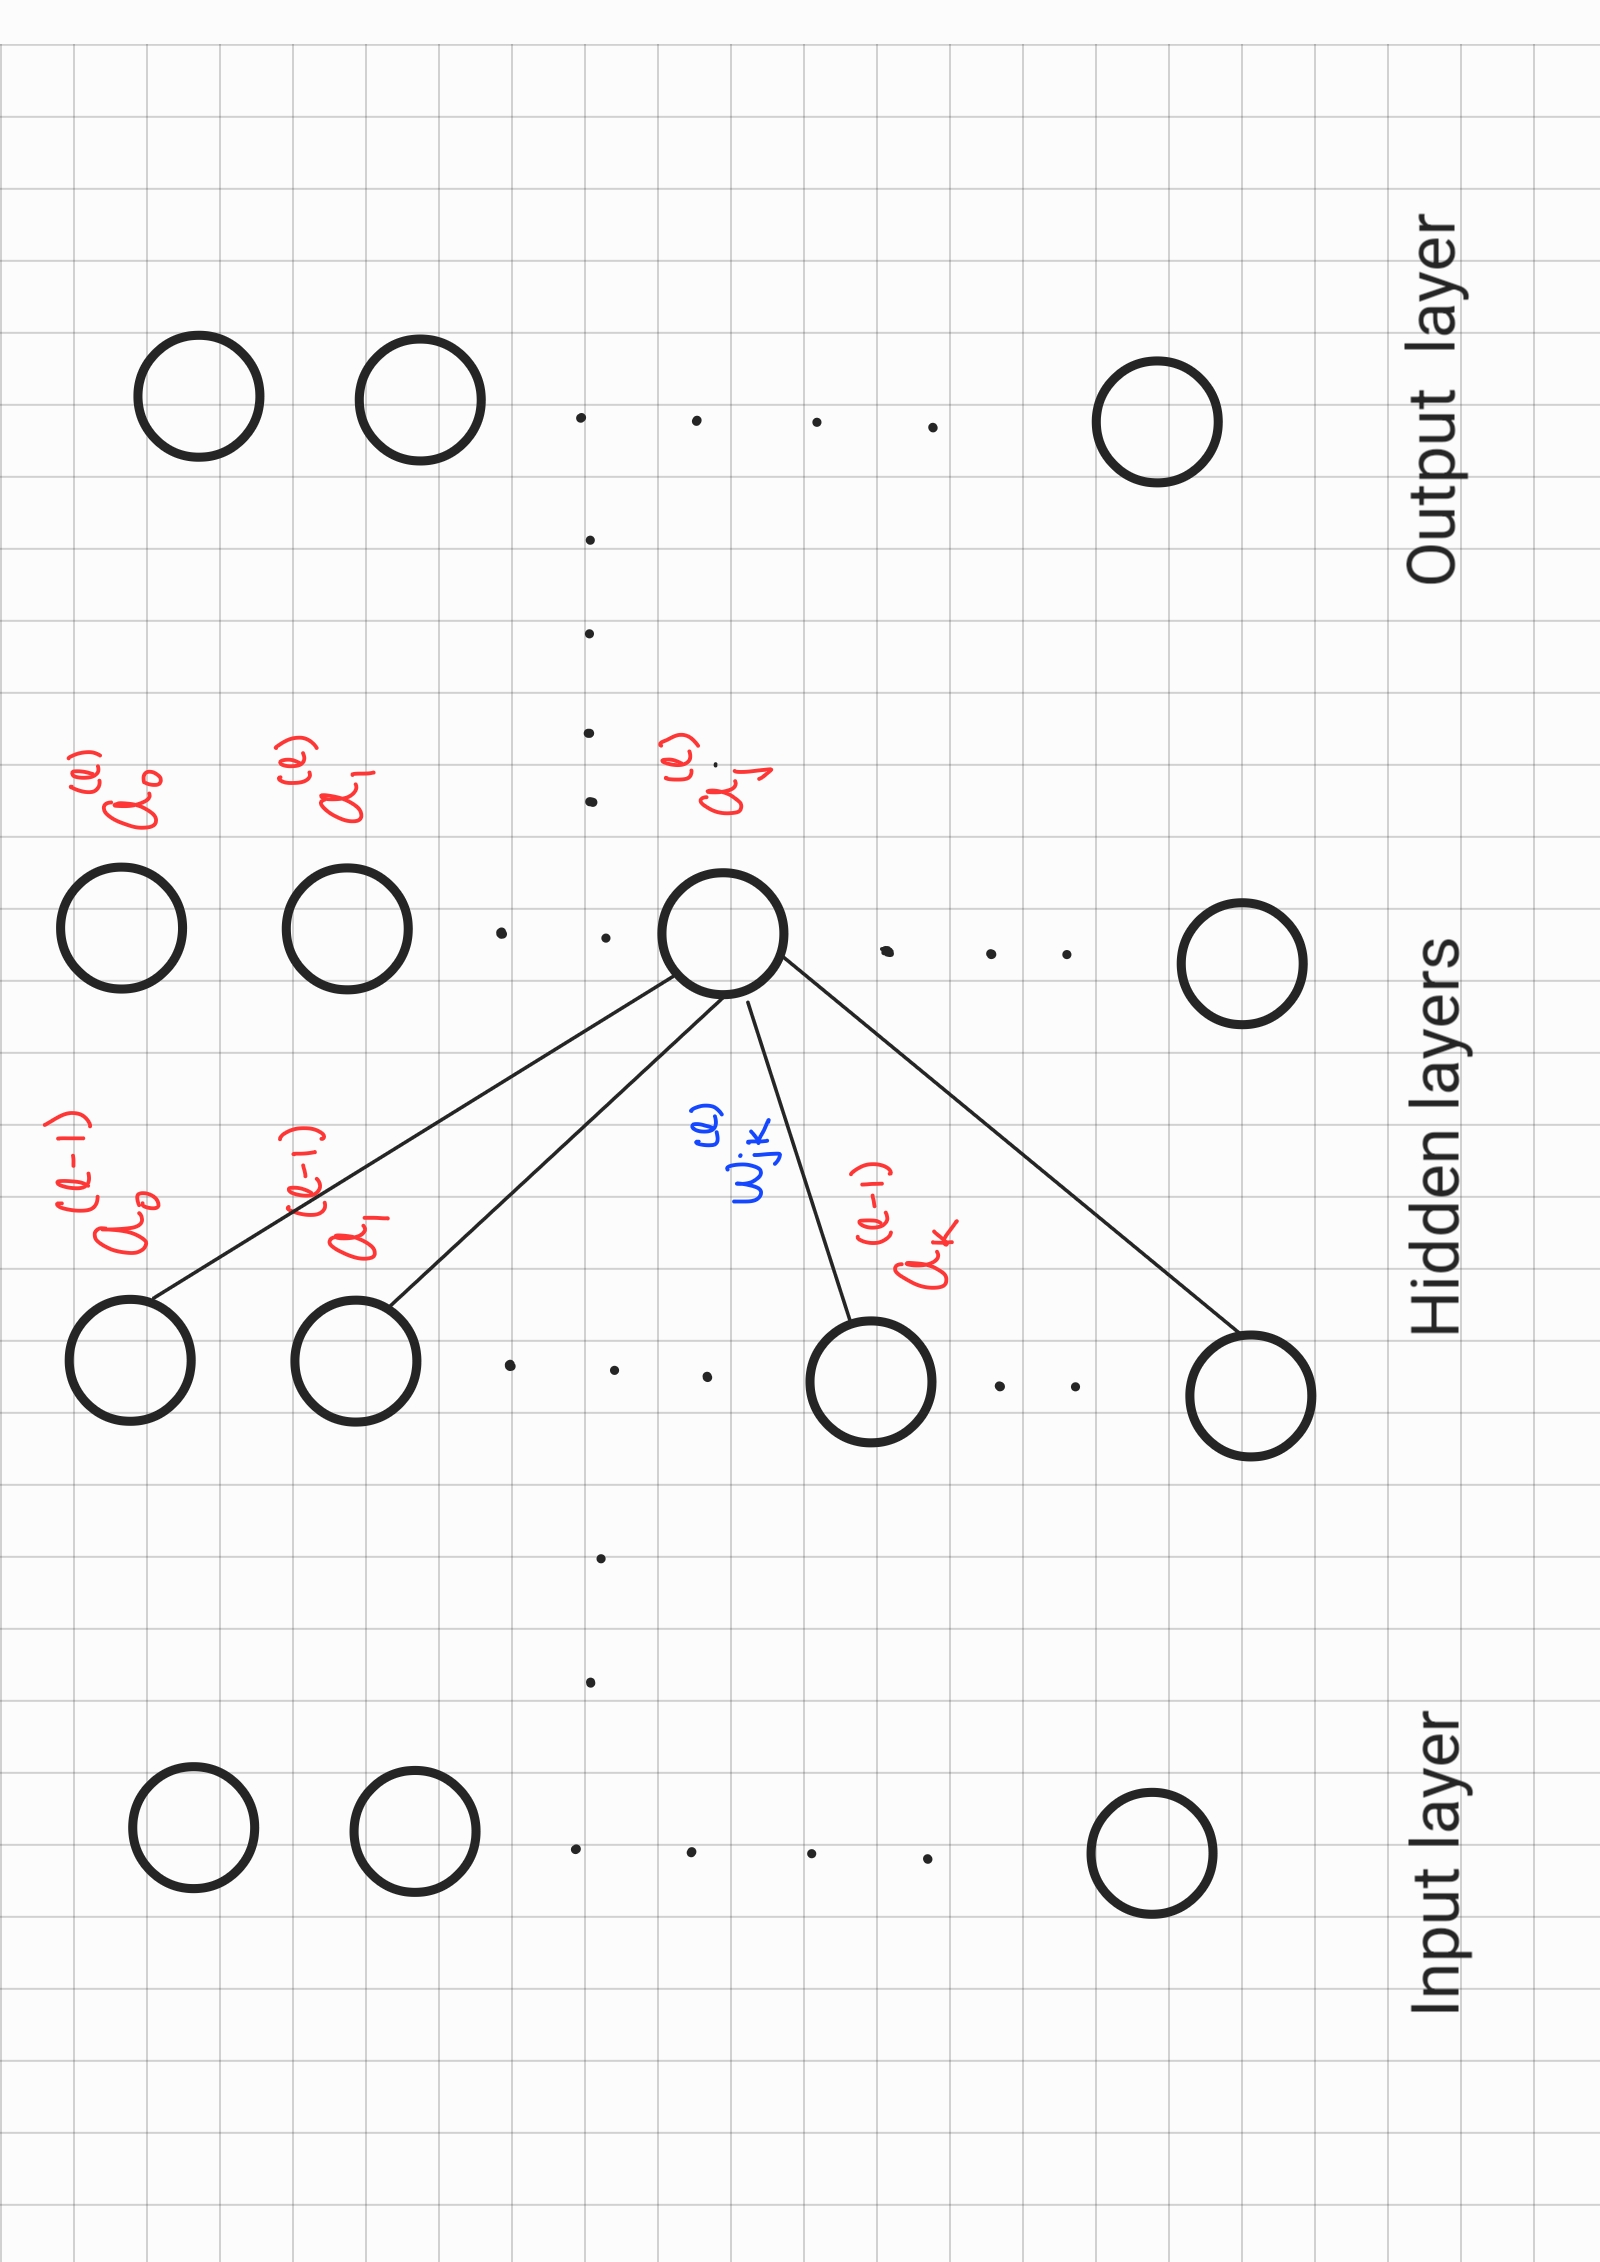
\includegraphics[width=.5\textwidth, angle = -90]{Figures/back_prop.jpg}
        \caption{Figure shows the notations assigned to different variables in a neural network while implementing backpropagation}
        \label{fig:back_p}
    \end{figure} 
We assign the following notations to weights, biases, weighted sums and activations of the network:
\begin{itemize}
    \item The activations are denoted by $a_j^{(l)}$ where the superscript represents the layer number and subscript represents the neuron number. The 
    layers are numbered starting from $l=1$ (the first layer i.e. input layer) while the neurons are numbered starting from $j=0$ (the first neuron).
    \item The weight for the connection between $k$th neuron of layer $l-1$ and $j$th neuron of layer $l$ is denoted by $w_{jk}^{(l)}$. The bias for the $j$th neuron in
    layer $l$ is denoted by $b_j^{(l)}$.
    \item The weighted sums are denoted by $z_j^{(l)}$ which are passed to an activation function resulting in activation $a_j^{(l)}$.
\end{itemize}
We have the following expressions for the cost function (for one training example), activations and weighted sums:
$$C_0 = \sum_{j=0}^{n_L -1} (a_j^{(L)} - y_j)^2, \quad a_j^{(l)} = \sigma(z_j^{(l)}), \quad z_j^{(l)} = \sum_{k=0}^{n_{l-1} -1} w_{jk}^{(l)}a_k^{(l-1)} + b_j^{(l)}$$
We can now derive the gradients following the chain-rule. We start by first calculating the gradients for the last layer,
\begin{equation}
    \label{eq:bp_eq_d}
    \begin{aligned}
        &\frac{\partial C_0}{\partial w_{jk}^{(L)}} = \frac{\partial z_j^{(L)}}{\partial w_{jk}^{(L)}} \frac{\partial a_j^{(L)}}{\partial z_j^{(L)}}\frac{\partial C_0}{\partial a_j^{(L)}}\\
        &\frac{\partial C_0}{\partial b_j^{(L)}} = \frac{\partial z_j^{(L)}}{\partial b_j^{(L)}} \frac{\partial a_j^{(L)}}{\partial z_j^{(L)}}\frac{\partial C_0}{\partial a_j^{(L)}}
    \end{aligned}
\end{equation}
We also derive the gradient with respect to activations in the second-last layer,
$$\frac{\partial C_0}{\partial a_k^{(L-1)}} = \sum_{j=0}^{n_{L} -1} \frac{\partial z_j^{(L)}}{\partial a_k^{(L-1)}} \frac{\partial a_j^{(L)}}{\partial z_j^{(L)}}\frac{\partial C_0}{\partial a_j^{(L)}}$$
We can evaluate the gradients $\frac{\partial C_0}{\partial w_{jk}^{(L-1)}}$ and $\frac{\partial C_0}{\partial b_j^{(L-1)}}$ using $\frac{\partial C_0}{\partial a_j^{(L-1)}}$. In this way we can keep moving backwards in the network (hence the name backpropagation)
and find gradients on the way back.  Notice that the only major change we see in the expressions for gradients when moving to complex neural networks from simple networks is for $\frac{\partial C_0}{\partial a_k^{(L-1)}}$. 
This is attributed to that fact that now we have multiple neurons in each layer. A change in the activation, say $\frac{\partial C_0}{\partial a_k^{(L-1)}}$, can affect the cost through multiple paths.
In general, we can write the derivatives of cost/loss function with respect to weights and biases for neurons in any layer $l$ as,
\begin{equation}
    \label{eq:bp_eq}
    \begin{aligned}
        &\frac{\partial C_0}{\partial w_{jk}^{(l)}} = a_k^{(l-1)}\sigma'(z_j^{(l)}) \frac{\partial C_0}{\partial a_j^{(l)}}\\
        &\frac{\partial C_0}{\partial b_j^{(l)}} = \sigma'(z_j^{(l)}) \frac{\partial C_0}{\partial a_j^{(l)}}
    \end{aligned}
\end{equation}
where 
$$\frac{\partial C_0}{\partial a_k^{(l)}} = \sum_{j=0}^{n_{l+1} -1} w_{jk}^{(l+1)} \sigma'(z_j^{(l+1)}) \frac{\partial C_0}{\partial a_j^{(l+1)}} \quad \text{or} \quad  2(a_k^{(L)} - y_k) \ \text{when} \ l=L.$$
The backpropagation algorithm is generally combined with a learning algorithm like stochastic gradient descent to update weights and biases. Let us see how this works for a mini-batch of $m$ training examples:
\begin{enumerate}
    \item Input a set of training examples. 
    \item For each training example $x$: Set the corresponding input activation $a^{x,1}$ and perform the following steps:
    \begin{itemize}
        \item Feedforward: For each $l = 2,3,....L$, compute $z_j^{(l)} = \sum_{k=0}^{n_{l-1} -1} w_{jk}^{(l)} a_k^{(l-1)} + b_j^{(l)}$ and $a_j^{(l)} = \sigma (z_j^{(l)})$
        \item Compute gradients for the last layer: $$\frac{\partial C_x}{\partial a_j^{(L)}}, \frac{\partial C_x}{\partial w_{jk}^{(L)}}, \frac{\partial C_x}{\partial b_j^{(L)}}$$
        \item Backpropagate: for $l = L-1, L-2, ...., 2$ compute $$\frac{\partial C_x}{\partial a_j^{(l)}}, \frac{\partial C_x}{\partial w_{jk}^{(l)}}, \frac{\partial C_x}{\partial b_j^{(l)}}$$
    \end{itemize}
    \item Gradient descent: for each $l = L, L-1, ......, 2$ update weights and biases
        $$w_{jk}^l \rightarrow w_{jk}^l - \frac{\eta}{m} \sum_x \frac{\partial C_x}{\partial w_{jk}^{(l)}} $$
        $$b_j^l \rightarrow b_j^l - \frac{\eta}{m} \sum_x \frac{\partial C_x}{\partial b_j^{(l)}} $$
\end{enumerate}
\subsection{Why backpropagation is a fast algorithm ?}
In the last section, we have illustrated the procedure to find gradient of the cost function. At first glance, the backpropagation algorithm may
seem complicated since it involves a lot of steps and one has to be very careful about the notations. In reality, the backpropagation algorithm is very 
simple to implement and is considered one of the most efficient methods for computing gradients. Most of the terms like $a_k^{(l-1)}, w_{jk}^{(l+1)}$, in 
the expressions for gradients are already available to the network when making a forward pass; the rest, for example $\sigma'(z_j^{(l)})$ can be easily computed.
We can see the advantages of using backpropagation when we compare it to another popular method for calculating gradients. Let us denote (for simplicity) the cost function by $C(w,b)$ 
where $w$ are the weights $w_1,w_2,.....$ and $b$ are the biases $b_1,b_2,....$ of a network. We can use the fundamental definition of partial derivatives to approximate gradients,
\begin{equation}
    \label{eq:part_de}
    \frac{\partial C}{\partial w_j} \approx \frac{C(w + \epsilon e_j, b) - C(w,b)}{\epsilon}
\end{equation}
where $\epsilon > 0$ is a small positive number, and $e_j$ is a unit-vector in the $j-$th direction. In other words, we can compute $\frac{\partial C}{\partial w_j}$ by first 
calculating the cost $C$ for two slightly  different values of $w_j$ and then applying equation \eqref{eq:part_de}. We can use this approach to 
calculate derivatives with respect to all weight and biases of the network. This method is extremly easy to implement and certainly looks better than the chain-rule. Therefore, one
might be tempted to use this instead of backpropagation. Unfortunately, this method is extremely slow ! 

Suppose we have a million ($10^6$) weights and biases in a network. In order to get 
gradients using equation \eqref{eq:part_de}, we have to compute the cost $10^6 + 1$ times; once to compute $C(w)$ and $10^6$ times to calculate $C(w + \epsilon e_j, b)$ for different $j$'s. This is equivalent to making
$10^6 +1$ forward passes of the network. On the other hand, with backpropagation, we need to make just one forward pass and one backward pass to calculate all the gradients. The computational cost 
of the backward pass is similar to the forward pass since both involve similar computations. Therefore, rougly speaking, (for this example) the backpropagation method is a million times faster than the numerical gradient computation method (equation \eqref{eq:part_de}).
The backpropagation is also more accurate than the numerical gradient method. The expression for gradient used in equation \eqref{eq:part_de} is an approximation of gradients and depends on the value of $\epsilon$ whereas the expressions used in backpropagation are exact.
\subsection{Implementation of a neural network to classify digits}
We use the ideas discussed in the previous sections to write a code for implementing a neural network
which can classify hand-written digits. A jupyter notebook which illustrates how this neural network performs on MNIST test data set is available in \complementary{\theexample}.
%%%%%%%%%%% UAT %%%%%%%%%%%%%%%%%%%%%
\section{The universal approximation theorem}
Neural networks are mathematical functions. We use training data to look for suitable weights and biases
such that the neural network can map/obtain the underlying function from which the data is drawn. But, how can one
believe that a neural network have the capability of finding the underlying function. What is so special about the
neural network structure that after training it is able to give us great results on unseen data/ test data ? The answer to these
questions lies in the universal approximation theorem (UAT) proposed by George Cybenko in $1989$. 
George Cybenko gave a rigorous proof that feed-forward neural networks can approximate any continuous function defined on a compact set \cite{cybenko1989approximation}. To understand the 
proof of this theorem, one should be familiar with some concepts from measure theory and functional analysis. 
Let us first briefly go through the mathematical preliminaries.
\begin{itemize}
    \item Consier an $n$-dimensional unit cube, $I_n = [0,1]^n$. In the universal approximation theorem, the continuous
    functions that a neural network aims to approximate are defined on compacts sets, $I_n$ i.e. the domain of continuous
    functions is $I_n$. 
    \item Let $C(I_n)$ denote the space of continuous functions on $I_n$.
    For any function $f \in C(I_n), f : [0,1]^n \rightarrow \mathbb{R}$, one can define a suitable norm, 
    $\|f\| = \text{sup}_{x \in I_n} |f(x)|$ known as uniform/supremum norm. We can associate a dual space to $C(I_n)$ 
    defined as $C(I_n)^* = \{L : C(I_n) \rightarrow \mathbb{R}\}$ where $L$ is a linear operator \cite{kreyszig1991introductory}.
    \item UAT is defined for feed-forward neural networks having an input layer (with multiple neurons), one hidden layer and
    an output layer with only one neuron (see figure \ref{fig:ffnn_UAT}). Therefore, the functions generated by the neural network can be described as
    $$G(x) = \sum_{j=1}^{N} \alpha_j \sigma (w_j\cdot x + b_j), \quad w_j \in \mathbb{R}^n, \alpha_j, b_j \in \mathbb{R}, x \in I_n$$
    where $N$ is the number of neurons in the hidden layer. We can note that bias is not added to output from the hidden
    layer. Also the output is not passed to an activation function. We denote the set of functions of the form $G(x)$
    by $\mathcal{N}$. In the problem of hand-written digit recognition, we assumed that the activation function, $\sigma$ is logistic/sigmoid. 
    However, UAT was proved for a general class of activation functions. The actvation functions are assumed to be continuous and 
    discriminatory \cite{cybenko1989approximation}. 
\end{itemize} 
\begin{figure}[htbp]
    \centering
    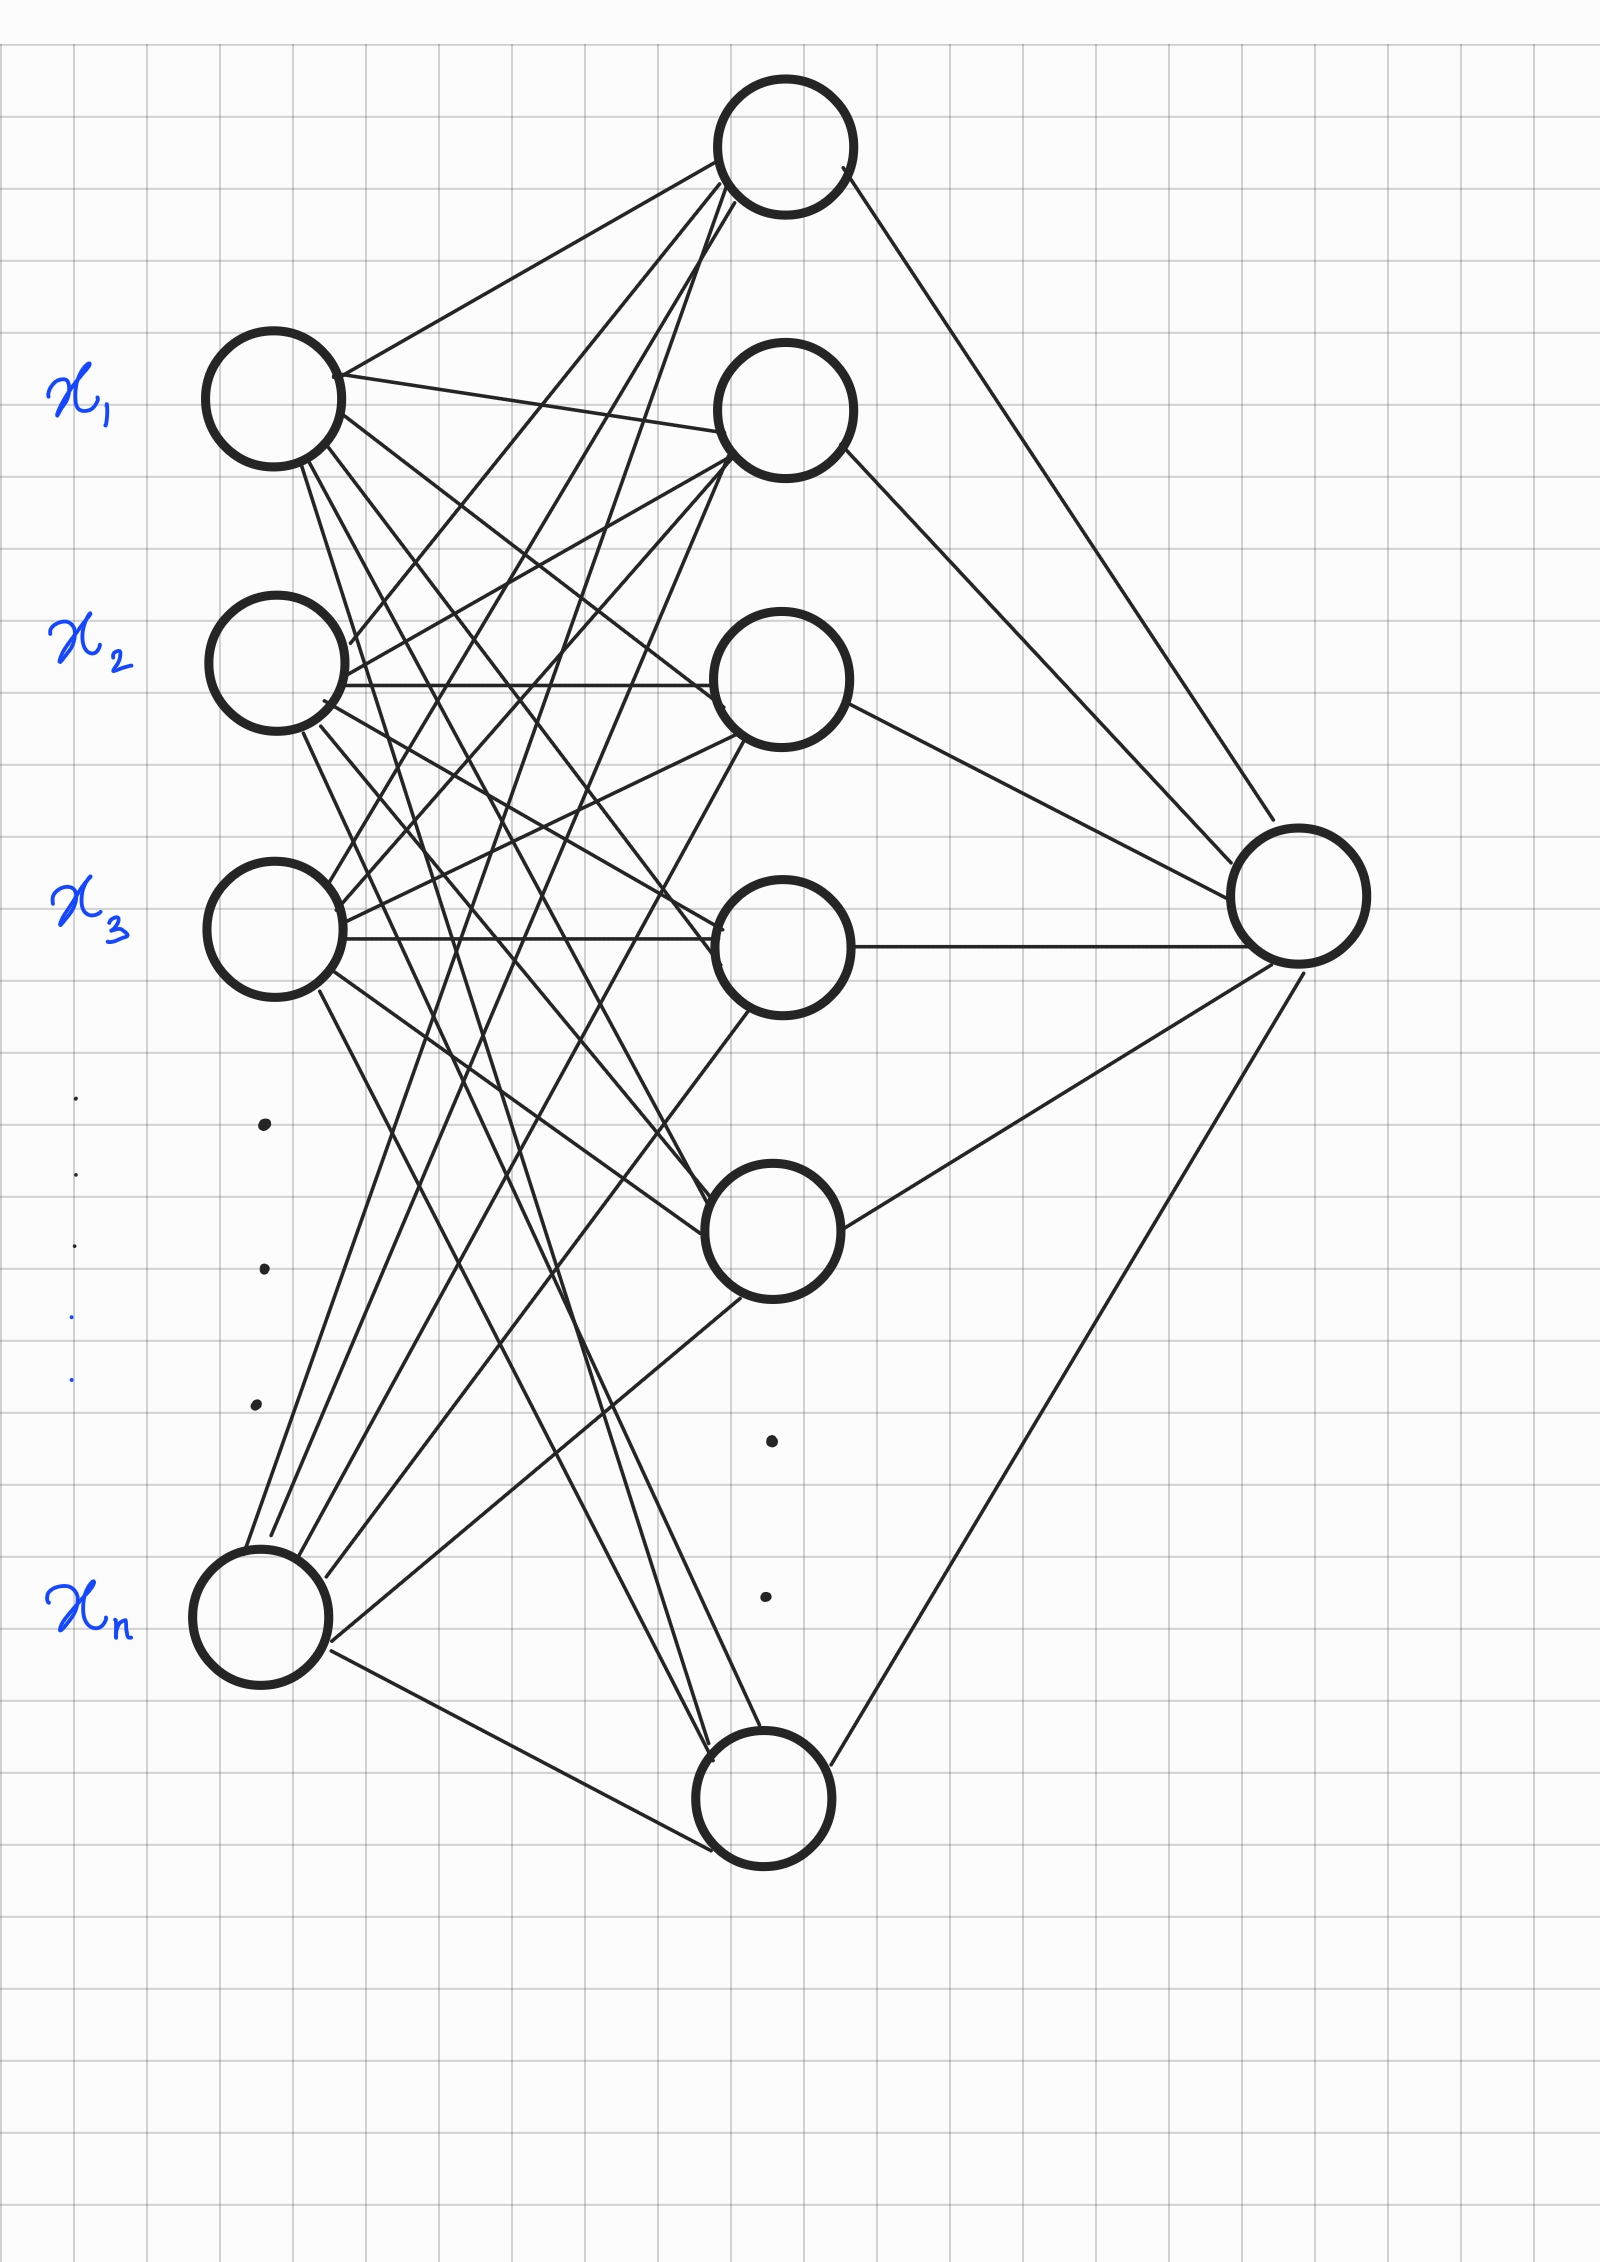
\includegraphics[width=.4\textwidth]{Figures/ffnn_UAT.jpg}
    \caption{A feed-forward neural network with an input layer (having multiple neurons), one hidden layer and an output layer (having only one neuron).}
    \label{fig:ffnn_UAT}
\end{figure}
\begin{definition}[Discriminatory function \cite{cybenko1989approximation}]
    We say that a function $\sigma$ is discriminatory if for a measure $\mu \in M(I_n)$ (where $M(I_n)$ is the space 
of finite, signed regular Borel measures on $I_n$) 
$$\int_{I_n} \sigma (\mathbf{w}\cdot\mathbf{x} + b) \ d\mu(\mathbf{x}) = 0$$
for all $\mathbf{w} \in \mathbb{R}^n$ and $b\in \mathbb{R}$ implies that $\mu = 0$.
\end{definition}
\begin{thm}[Universal approximation theorem \cite{cybenko1989approximation}]
    \label{thm:UAT}
    Let $\sigma$ be any continuous discriminatory function. Then the set $\mathcal{N}$ of functions of the form 
    $$G(x) = \sum_{j=1}^{N} \alpha_j \sigma (w_j\cdot x + b_j), \quad w_j \in \mathbb{R}^n, \alpha_j, b_j \in \mathbb{R}, x \in I_n$$
    are dense in $C(I_n)$. In other words, given any function $f \in C(I_n)$ and $\epsilon > 0$, there exists
    a $G(x) \in \mathcal{N}$ such that 
    $$\| G(x) - f(x)\| < \epsilon \ \text{for all} \ x \in I_n$$
\end{thm}
Before going into the proof of UAT, we will familiarize ourselves with some key ideas from measure theory \cite{tao2011introduction}, \cite{kyleUAT}.
\begin{itemize}
    \item Our aim to measure subsets of $I_n = [0,1]^n$. A collection $\sum$ of subsets of $I_n$ is called a 
    $\sigma$-algebra (note that this $\sigma$ has no relation to activation function $\sigma$)if 
    \begin{enumerate}
        \item $I_n \in \sum$
        \item If $A \in \sum$, then $A^c = I_n\backslash A \in \sum$
        \item If $A_1, A_2, .....$ is a countable collection of subsets of $\sum$ then $\bigcup^\infty A_i \in \sum$.
    \end{enumerate}
    \item Borel $\sigma$-algebra on $I_n$ is the smallest $\sigma$-algebra  containing all open sets in $I_n$. Sets in Borel $\sigma$-algebra 
    are called Borel sets.
    \item A finite signed Borel measure $\mu$ on $I_n$ is a real valued  function, $\mu : \sum \rightarrow \mathbb{R}$  (where
    $\sum$ is a Borel $\sigma$-algebra defined on $I_n$) such that 
    \begin{enumerate}
        \item $\mu (\phi) = 0$
        \item $\mu (\bigcup_{i=1}^{\infty} A_i) = \sum_{i=1}^{\infty} \mu(A_i), A_i \ \text{are disjoint sets}$
        \item $\mu(A_i) < \infty$
    \end{enumerate}
    \item A Borel measure is regular if 
    \begin{align*}
        &\mu(A) = \text{sup} \{\mu(K) | K \subseteq A, K \ \text{is compact}\} \\
        &\mu(A) = \text{inf} \{\mu(U) | A \subseteq U, U \ \text{is open}\}
    \end{align*}
    In other words, what regular means is every measurable set can be approximated from above by open measurable 
    sets and from below by compact measurable sets. 
    \item We define $M(I_n)$ as the set of all finite signed regular Borel measures on $I_n$.
\end{itemize}
The proof of UAT also uses ideas from Hahn-Banach theorem and Riesz representation theorem. These theorems 
have various equivalent versions. We now define the versions which we will refer to later in the proof. 
\begin{thm}[Riesz representation theorem \cite{rudin}]
    \label{thm:RR}
    If $K \subset \mathbb{R}^d$ is a compact set, then every linear functional $L$ defined on
    $C(K)$ can represented by a unique regular signed Borel measure $\mu \in M(K)$ in the sense that,
    $$L(f) = \int_K f \ d\mu$$
    where $f: K \rightarrow \mathbb{R}$.
\end{thm}
\begin{thm}[Hahn-Banach theorem, \cite{rudin}]
    \label{thm:HB}
    Let $M$ be a linear subspace of a normed linear space $X$, and $f_0 \in X$. Then $f_0$ is 
    in the closure $\overline{M}$ of $M$ if and only if there is no bounded linear functional 
    $L$ on $X$ such that $L(f) = 0 $ for all $f\in M$ but $L(f_0) \neq 0$.
\end{thm}
We now give the proof of universal approximation theorem \ref{thm:UAT}.
\begin{proof}
   $C(I_n)$ is a vector space equipped with a supremum norm and hence is a normed vector space. It is
   clear that the set formed by functions of the form $G(x)$ is a subset of $C(I_n)$ i.e. $\mathcal{N} \subset C(I_n)$.
   We claim that $\mathcal{N}$ is also a linear subspace of $C(I_n)$. This is true due to the fact that if 
   we take two functions $G_1(x), G_2(x) \in \mathcal{N}$, we can always find a function $G_3(x) \in \mathcal{N}$ such that 
   $G_3(x) = \alpha G_1(x) + \beta G_2(x)$ for all $\alpha, \beta \in \mathbb{R}$. Our next claim is that the closure of 
   $\mathcal{N}$ is all of $C(I_n)$ i.e. $\mathcal{N}$ is dense in $C(I_n)$. We prove this by contradiction \cite{rudin}. 

   Assume that the closure of $\mathcal{N}$, $\overline{\mathcal{N}}$ is not all of $C(I_n)$ i.e. 
   $\overline{\mathcal{N}} \neq C(I_n)$. It can be proved (refer any standard functional analysis book) that $\overline{\mathcal{N}}$
   is a closed proper subspace of $C(I_n)$.  By Hahn Banach theorem \ref{thm:HB}, there exists a bounded 
   linear functional on $C(I_n)$, let's call it $L$, with the property that $L \neq 0$ but $L(\overline{\mathcal{N}}) = L(\mathcal{N}) = 0$.
   By following Riesz representation theorem \ref{thm:RR}, we can write this linear operator, $L$ as 
   $$L(h) = \int_{I_n} h(x) \ d\mu(x)$$
   for some $\mu \in M(I_n) \ \forall h \in C(I_n)$. Since this operator returns zero for all elements of $\mathcal{N}$,
   we must have for all $w \in \mathbb{R}^n, b \in \mathbb{R}$ 
   $$\int_{I_n} \sigma (w \cdot x + b) \ d\mu(x) = 0.$$
   However, we assumed that $\sigma$ is a discriminatory functions therefore this condition implies that $\mu =0$. This contradicts our initial assumption that 
   $\overline{\mathcal{N}} \neq C(I_n)$ which led to $L \neq 0 \equiv \mu \neq 0$ via Hahn Banach theorem. Hence, the subspace $\mathcal{N}$ must be dense in $C(I_n)$. 
\end{proof}
The universal approximation theorem gives us confidence that neural networks can indeed approximate any continuous function 
provided that the activation function is continuous and discriminatory. However, it is not clear how to build activation functions which are 
discriminatory.
\begin{definition}
    \label{def:sig}
    We say that $\sigma$ is sigmoidal if 
    \begin{equation*}
        \sigma(t) \rightarrow 
         \begin{cases}
           1 &\quad \text{as} \ \ t\rightarrow +\infty\\
           0 &\quad \text{as} \ \ t\rightarrow -\infty.
         \end{cases}
    \end{equation*}
\end{definition}
\begin{lemma}
    \label{lem:sig}
    Any continuous sigmoidal function is discriminatory.
\end{lemma}
\begin{proof}
    Refer \cite{cybenko1989approximation}.
\end{proof}
The lemma \ref{lem:sig} gives us a way to build suitable activation functions. In fact, the sigmoid/logistic function we used as an activation function
in the neural network for solving hand-written recognition problem satisfies the conditions of definition \ref{def:sig} and is therefore, discriminatory. Although 
logistic function is monotonically increasing, no monotonicity is required by definition \ref{def:sig}.
% Chapter 1
% !TeX spellcheck = en_US 
\chapter{Modern Machine Learning} % Main chapter title

\label{Chapter4} % For referencing the chapter elsewhere, use \ref{Chapter1} 
\setcounter{chapter}{4}
%----------------------------------------------------------------------------------------


% Chapter 1
% !TeX spellcheck = en_US 
\chapter{Modern Mathematical Machine Learning} % Main chapter title

\label{Chapter5} % For referencing the chapter elsewhere, use \ref{Chapter1} 

%----------------------------------------------------------------------------------------

\printbibliography[heading=bibintoc]
% Add more Chapters as needed...

\end{document}
